% -------------------------------------------------------------------------------
% Establish page structure & font.
\documentclass[12pt]{report}

\usepackage[total={6.5in, 9in},
	left=1in,
	right=1in,
	top=1in,
	bottom=1in,]{geometry} % Page structure

\usepackage{graphicx} % Required for inserting images
\graphicspath{{../../.images/}} % Any additional images I use (BCU logo, etc) are from here.

\usepackage[utf8]{inputenc} % UTF-8 encoding
\usepackage[T1]{fontenc} % T1 font
\usepackage{float}  % Allows for floats to be positioned using [H], which correctly
                    % positions them relative to their location within my LaTeX code.
\usepackage{subcaption}

% -------------------------------------------------------------------------------
% Declare biblatex with custom Harvard BCU styling for referencing.
\usepackage[
    useprefix=true,
    maxcitenames=3,
    maxbibnames=99,
    style=authoryear,
    dashed=false, 
    natbib=true,
    url=false,
    backend=biber
]{biblatex}

% Additional styling options to ensure Harvard referencing format.
\renewbibmacro*{volume+number+eid}{
    \printfield{volume}
    \setunit*{\addnbspace}
    \printfield{number}
    \setunit{\addcomma\space}
    \printfield{eid}}
\DeclareFieldFormat[article]{number}{\mkbibparens{#1}}

% Declaring both bib sources.
% Pipeline is the original one copied from draft pipeline, Report is new for this.
% This is because pipeline.bib is over a thousand lines long.
\addbibresource{Pipeline.bib}
\addbibresource{Report.bib}

% -------------------------------------------------------------------------------
% To prevent "Chapter N" display for each chapter
\usepackage[compact]{titlesec}
\usepackage{wasysym}
\usepackage{import}

\titlespacing*{\chapter}{0pt}{-2cm}{0.5cm}
\titleformat{\chapter}[display]
{\normalfont\bfseries}{}{0pt}{\Huge}

% -------------------------------------------------------------------------------
% Custom macro to make an un-numbered footnote.

\newcommand\blfootnote[1]{
    \begingroup
    \renewcommand\thefootnote{}\footnote{#1}
    \addtocounter{footnote}{-1}
    \endgroup
}

% -------------------------------------------------------------------------------
% Fancy headers; used to show my name, BCU logo and current chapter for the page.
\usepackage{fancyhdr}
\usepackage{calc}
\pagestyle{fancy}

\setlength\headheight{37pt} % Set custom header height to fit the image.

\renewcommand{\chaptermark}[1]{%
    \markboth{#1}{}} % Include chapter name.


% Lewis Higgins - ID 22133848           [BCU LOGO]                [CHAPTER NAME]
\lhead{Lewis Higgins - ID 22133848~~~~~~~~~~~~~~~
\includegraphics[width=1.75cm]{BCU}}
\fancyhead[R]{\leftmark}

% ------------------------------------------------------------------------------
% Used to add PDF hyperlinks for figures and the contents page.

\usepackage{hyperref}

\hypersetup{
    colorlinks=true,
    linkcolor=black,
    filecolor=magenta,
    urlcolor=blue,
    citecolor=black,
}

% ------------------------------------------------------------------------------
\usepackage{xcolor} 
\usepackage{colortbl}
\usepackage{longtable}
\usepackage{amssymb}
% ------------------------------------------------------------------------------
\usepackage{tcolorbox}
\newcommand{\para}{\vspace{7pt}\noindent}
% -------------------------------------------------------------------------------

\title{Data Management and MLOps Activities Log Report}
\author{Lewis Higgins - Student ID 22133848}
\date{December 2024}

% -------------------------------------------------------------------------------

\begin{document}


\makeatletter
\begin{titlepage}
    \begin{center}
        
\includegraphics[width=0.7\linewidth]{BCU}\\[4ex]
        {\huge \bfseries CMP6230 - Assignment 2}\\[2ex]
        {\large \bfseries  \@title}\\[50ex]
        {\@author}\\[2ex]
        {CMP6230 - Data Management and Machine Learning Operations}\\[2ex]
        {Module Coordinator: Sima Iranmanesh}\\[10ex]
    \end{center}
\end{titlepage}
\makeatother
\thispagestyle{empty}
\newpage


% Page counter trick so that the contents page doesn't increment it.
\setcounter{page}{0}

\tableofcontents
\thispagestyle{empty}

\chapter*{Introduction}
\addcontentsline{toc}{chapter}{Introduction}
% UPDATE INTRO BECAUSE THE REPORT ISN'T JUST A PLAN ANYMORE.
This report aims to design and document a five-stage Machine Learning Operations pipeline, from the initial 
data ingestion to the monitoring of the produced model, beginning 
with the identification of three candidate datasets for the pipeline to be conducted with, and continuing 
into descriptions of what each stage of the pipeline consists of, and how it will be implemented with the
one chosen dataset using a wide variety of software that is also used within industry. When this plan 
is implemented at a later stage, it will provide a clear framework to create an automated MLOps pipeline
with continuous integration and deployment.

% Importing the sections from the original report here.
\chapter{Candidate Data Sources}
For the first stage of the pipeline, data ingestion, three data sources will be identified in order to find 
the one that would be most optimal for the production and deployment of a machine learning model to complete 
a supervised learning task.

\section{Candidate 1 - Indian Liver Patient Dataset}
This dataset \autocite{bendi_ramana_ilpd_2022} consists of real data sourced from hospitals northeast of Andhra Pradesh in India. It was obtained from the
UCI Machine Learning Repository, and has been previously used by \textcite{straw_investigating_2022} in their analysis of sex-related bias in supervised learning models. The UCI ML Repository is a popular host of datasets used by students, 
educators and researchers worldwide for machine learning \autocite{uci_machine_learning_repository_about_nodate}, and hosts these datasets 
on the cloud for public download and usage, as long as credit is given.

\begin{figure}[H]
    \centering
    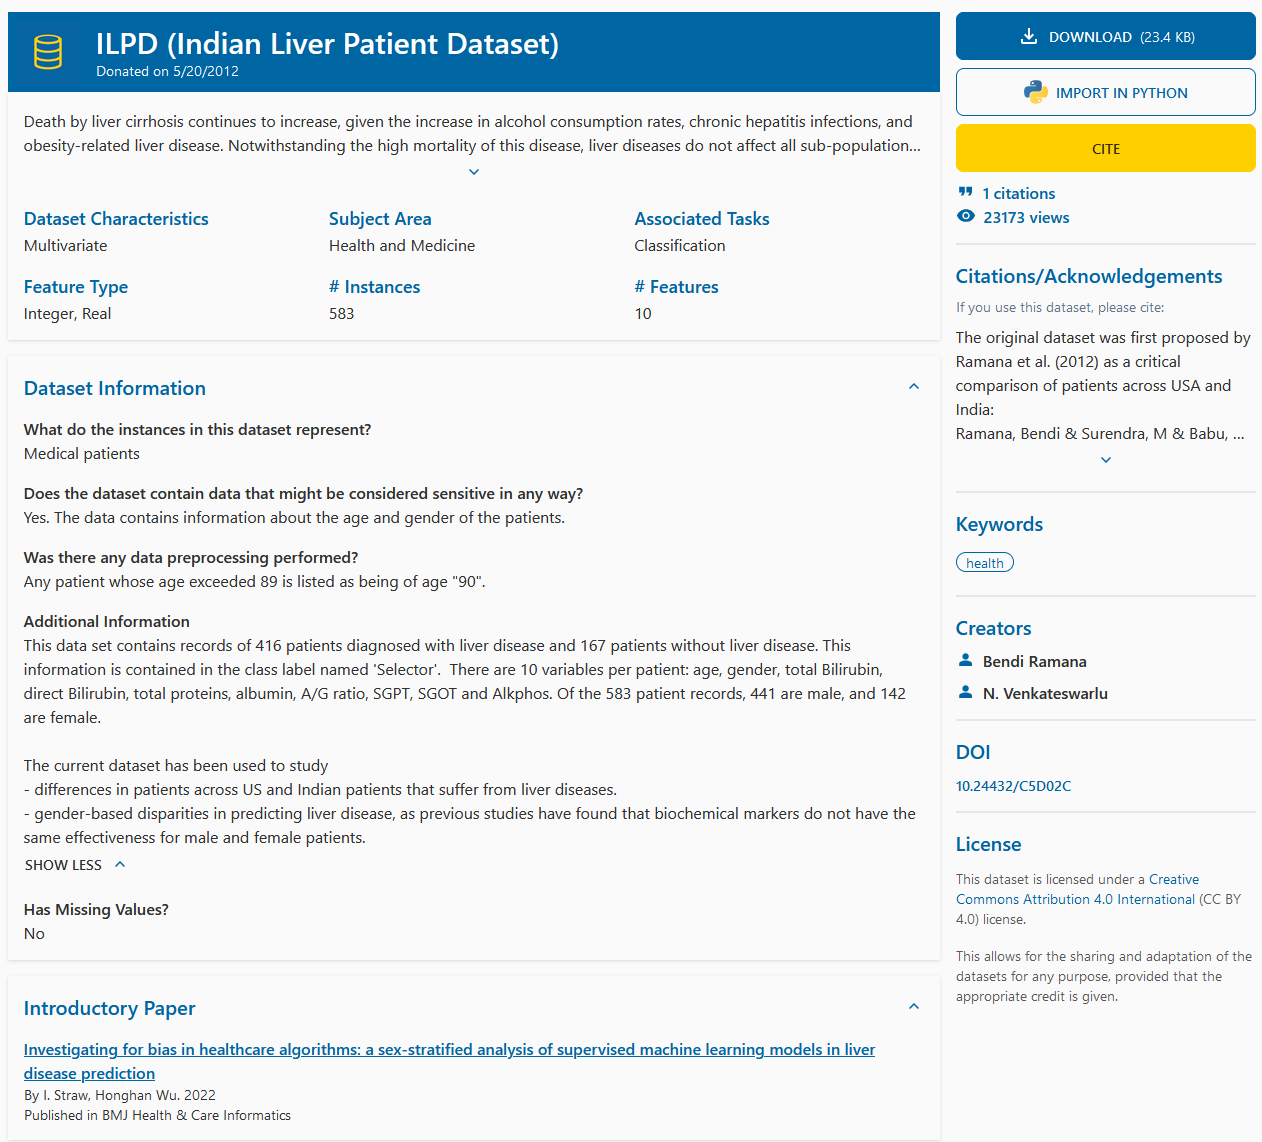
\includegraphics[width=.75\linewidth]{Draft Pipeline/ILPD-UCI.png}
    \caption{A snapshot of the dataset's UCI repository page.}
    \label{fig:ILPD-UCI}
\end{figure}

This dataset in particular aims to assist in the diagnosis of liver
disease due to increasing mortality rates from conditions like liver cirrhosis, and contains 584 records with 10 features
as well as the "Selector" classification column, where those without liver disease are classed as 1, and those with liver disease 
are classed as 2. For the purposes of the ML model, these can be changed to 0 and 1 respectively. 
The dataset is a single flat-file Comma-Separated Values (CSV) file, which stores data by separating each column with commas
and each row with line breaks. This CSV file uses a One Big Table (OBT) schema, as seen in the entity relationship diagram 
in Figure \ref{fig:ILPD-ERD}, wherein all of the data within this dataset is stored in a single table. 
The OBT schema is a denormalised schema that is useful for simple querying due to there being no need for table joins. 
However, it is prone to data duplication and redundancy, which can increase necessary storage requirements.

Descriptions of the columns in the dataset, as well as the associated data types, can be found in Table \ref{tab:ILPD-Types}.

\begin{figure}[H]
    \centering
    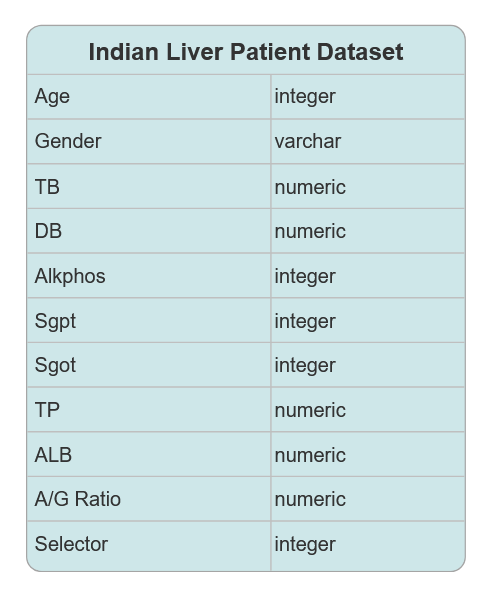
\includegraphics[width=.75\linewidth]{Draft Pipeline/ILPD-ERD.png}
    \caption{An entity relationship diagram of the Indian Liver Patient Dataset.}
    \label{fig:ILPD-ERD}
\end{figure}


A minor issue with this file is that it has no headers in its CSV file, meaning that when imported, Pandas will interpret the first 
row of data as the names of the columns, though this can be combated by adding the "names" argument when calling Pandas' "read\_csv" function,
seen below in Figure \ref{fig:pandasNames}. 

\begin{figure}[H]
    \centering
    \begin{subfigure}{0.75\textwidth}
       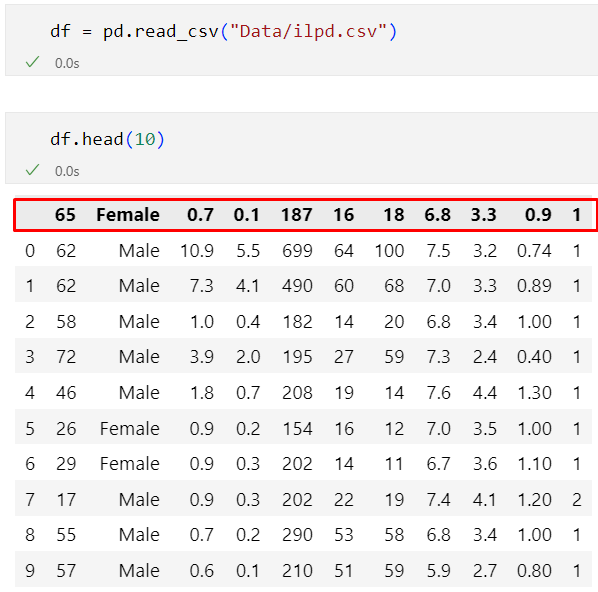
\includegraphics[width=1\linewidth]{Draft Pipeline/pandasNoNames.png}
       \caption{Importing without supplying column names.}
       \label{fig:pandasNames} 
    \end{subfigure}
    
    \begin{subfigure}{1\textwidth}
       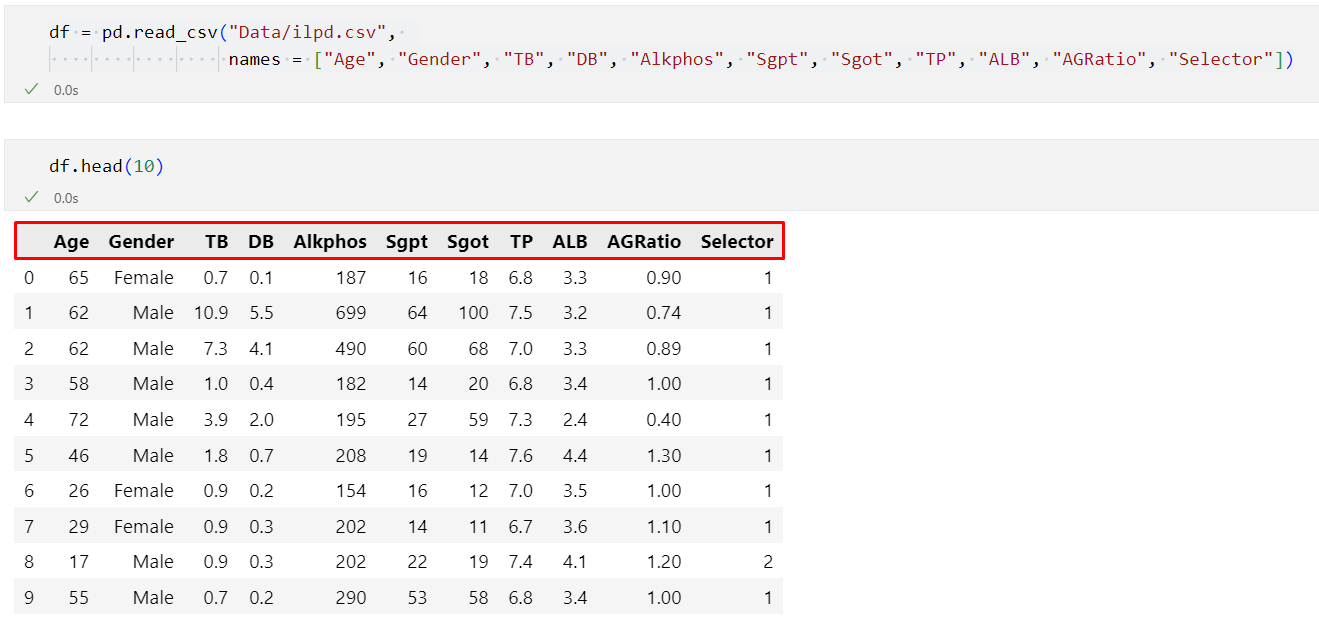
\includegraphics[width=1\linewidth]{Draft Pipeline/pandasNames.png}
       \caption{Importing with the column names.}
       \label{fig:PN2}
    \end{subfigure}
    \caption{Importing and viewing the head of the erroneous CSV using Pandas. The column headers are highlighted in a red box.}
\end{figure}

A preliminary analysis of the file to ascertain the data types of each column, seen in Figure \ref{fig:ILPD-DTypes}, also revealed that there were 4 missing values in the A/G ratio column.
It is possible that these missing values could be imputed rather than deleted, as it may be possible to calculate what the A/G ratio of these rows would have been in the 
Data Preprocessing stage of a pipeline.

\begin{figure}[H]
    \centering
    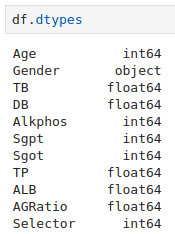
\includegraphics[width=.3\linewidth]{Draft Pipeline/pandas/ILPD-DTypes.png}
    \caption{The data types of the Indian Liver Patient Dataset.}
    \label{fig:ILPD-DTypes}
\end{figure}

\begin{figure}[H]
    \centering
    \begin{subfigure}{0.75\textwidth}
        \centering
       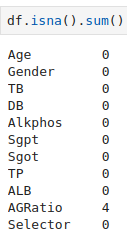
\includegraphics[width=0.3\linewidth]{Draft Pipeline/pandas/ILPD-NA.png}
       \caption{Four missing values are identified.}
       \label{fig:NAs1} 
    \end{subfigure}
    
    \begin{subfigure}{1\textwidth}
        \centering
       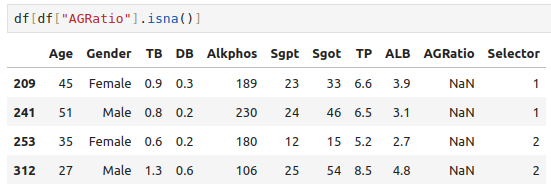
\includegraphics[width=1\linewidth]{Draft Pipeline/pandas/ILPD-NAValues.png}
       \caption{The four rows in question.}
       \label{fig:NAs2}
    \end{subfigure}
    \caption{The identification of four missing values in the A/G ratio column.}
\end{figure}


\begin{table}[H]
    \centering
        \begin{tabular}{ |p{0.2\textwidth}| p{0.4\textwidth}| p{0.2\textwidth}|}
            \hline
            \cellcolor{blue!25}Column & \cellcolor{blue!25}Description & \cellcolor{blue!25}Measurement level\\
            \hline
            Age & The patient's age. \textbf{Ages of 90 or over were listed as 90 before this dataset was published,
            which could introduce a bias in the machine learning model.} 
            & Ratio\\
            \hline
            Gender & The patient's gender, either "Male" or "Female". & Nominal\\
            \hline
            TB & Total bilirubin. Bilirubin is a substance produced by the liver, and a high presence of it may be indicative of
            liver problems \autocite{mayo_clinic_bilirubin_nodate}. & Ratio\\
            \hline
            DB & Direct bilirubin. This is a slightly different form of bilirubin that is formed after the liver has processed it.
            & Ratio\\
            \hline
            Alkphos & Levels of alkaline phosphate - an enzyme in the body produced by the liver. Too much may indicate liver disease. \autocite{clevelandclinic_alkaline_nodate}
            & Ratio\\
            \hline
            Sgpt & Another enzyme found in the liver, where too much can indicate liver problems.
            & Ratio\\
            \hline
            Sgot & Levels of AST in the blood, where too much indicates liver problems.
            & Ratio\\
            \hline
            TP & Total proteins.
            & Ratio\\
            \hline
            ALB & Albumin - a protein in blood plasma. Too little of this may indicate liver problems.
            & Ratio\\
            \hline
            A/G Ratio & The ratio of albumin to globulin, which is another blood protein.
            & Ratio % IS THIS RATIO?
            \\
            \hline
            Selector & The classifier, indicating if the person has liver disease. The target column for the ML model.
            & Nominal\\
            \hline
    \end{tabular}
    \caption{The descriptions of each column in the Indian Liver Patient Dataset.}\label{tab:ILPD-Types}
\end{table}

This dataset could be used to solve a binary classification problem using the ten predictor 
variables and the ground truth Selector column, which will be used in measuring the accuracy of the model. There is a clear 
positive purpose for developing such a model; as previously mentioned, mortality rates from liver disease are high, and an early
diagnosis that could leverage the power of machine learning can greatly enhance the odds of successful treatment.

\pagebreak

\section{Candidate 2 - Spotify Likes Dataset}
This dataset \autocite{vergnou_spotify_nodate} was sourced from \href{https://www.kaggle.com/datasets}{Kaggle}, a platform similar to the UCI ML repository in its 
purpose for students and researchers that acts as a search engine for datasets, but also allows its users to host competitions, upload their machine learning models, and also upload 
their own Python notebooks \autocite{kaggle_kaggle_nodate}. This dataset is stored on their servers on the cloud, and is free to download and use under a 
Creative Commons Public Domain license \autocite{creative_commons_deed_nodate}.

\begin{figure}[H]
    \centering
    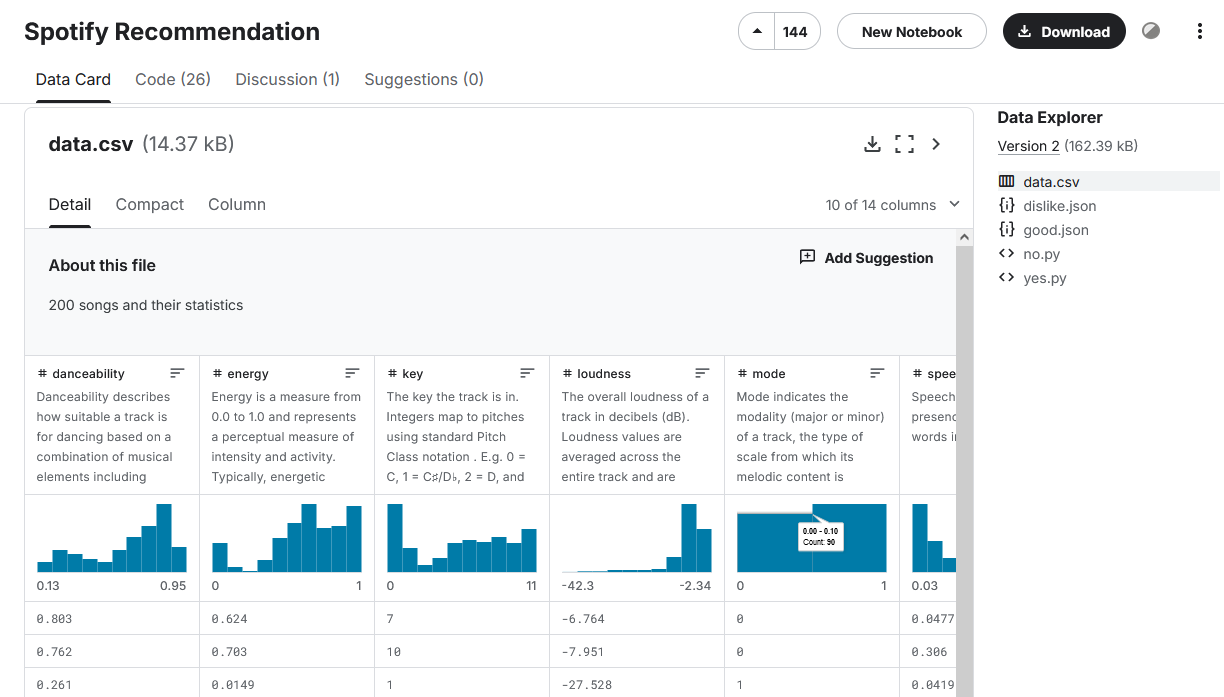
\includegraphics[width=.75\linewidth]{Draft Pipeline/Spotify-Kaggle.png}
    \caption{A snapshot of the Spotify dataset's Kaggle page.}
    \label{fig:Spotify-Kaggle}
\end{figure}

The data itself is split over 
two JavaScript Object Notation (JSON) files, but also fully present in an included CSV file, with all three utilising a One Big Table schema. The 
download also includes two Python files, which have the JSON data stored in Python dictionaries for ease of access, though these will not be used in 
this brief analysis. JSON files store data in \textbf{key-value pairs}, such as in the example snippet of this dataset depicted in Figure \ref{fig:spotifySnippet}.  

\begin{figure}[H]
    \centering
    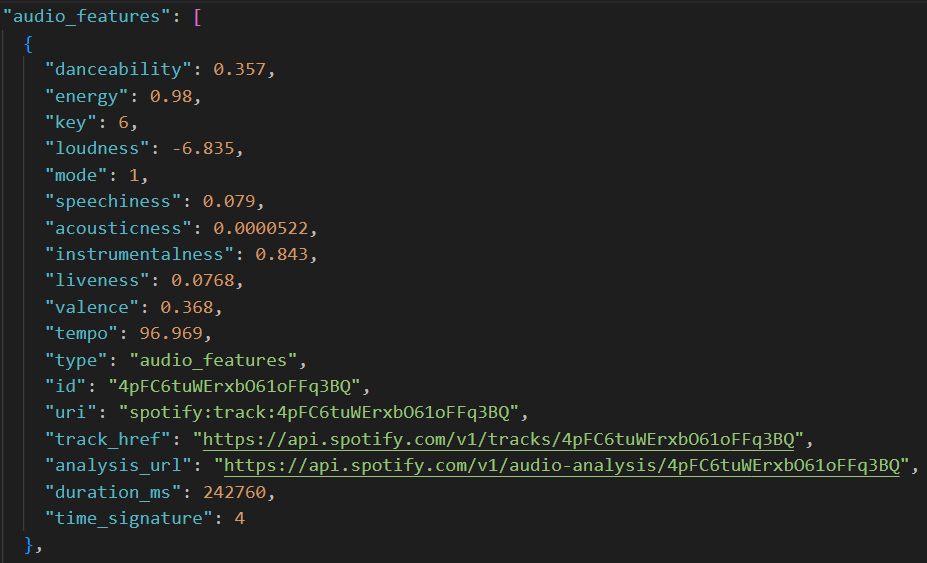
\includegraphics[width=.75\linewidth]{Draft Pipeline/spotifySnippet.png}
    \caption{A snippet of the JSON data, viewed in Visual Studio Code.}
    \label{fig:spotifySnippet}
\end{figure}

Every row in the JSON files is part of the single "audio\_features" key, and each new row is separated by curly braces \{\}. Each column is then given as a 
key-value pair, such as the first row in Figure \ref{fig:spotifySnippet}, where "danceability" is the key, and 0.352 is the associated value.

\noindent This dataset does consist of real data, sourced from the author's personal liked songs directly via the 
\href{https://developer.spotify.com/documentation/web-api}{Spotify API}. There are 195 rows of data, with 100 liked songs, and 95 disliked songs.
Liked and disliked songs are separated into two JSON files, named "dislike" and "good". The two JSON files have 18 features, as depicted in Figure 
\ref{fig:JSON-ERD}. 

\begin{figure}[H]
    \centering
    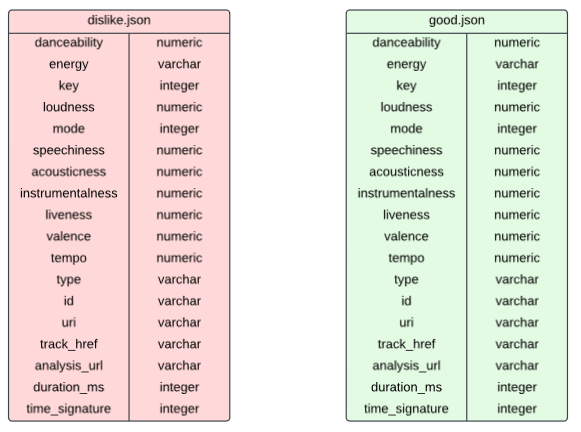
\includegraphics[width=.75\linewidth]{Draft Pipeline/SpotifyJSON-ERD.png}
    \caption{An entity relationship diagram of the two JSON files.}
    \label{fig:JSON-ERD}
\end{figure}

This dataset has been used to create machine learning models before, most notably by its own author, who has a public GitHub repository 
showcasing their work \autocite{brice-vergnou_brice-vergnouspotify_recommendation_2024}. 
Before publicising this data, however, the author had done some preprocessing of their own, having included the additional CSV file,
produced as a result of merging the two JSON files into one CSV and removing unnecessary columns, as depicted in Figure \ref{fig:Spotify-ERD}.
Therefore, my preliminary Pandas analysis of the data types and missing values will only be performed on this CSV, seen in Figures \ref{fig:Spotify-DTypes}
and \ref{fig:Spotify-NA}.

\begin{figure}[H]
    \centering
    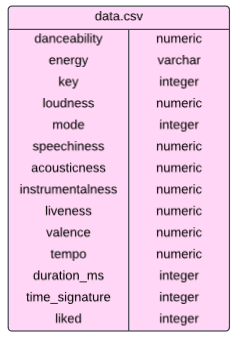
\includegraphics[width=.5\linewidth]{Draft Pipeline/Spotify-ERD.png}
    \caption{An entity relationship diagram of the author's preprocessed CSV file.}
    \label{fig:Spotify-ERD}
\end{figure}

\begin{figure}[H]
    \centering
    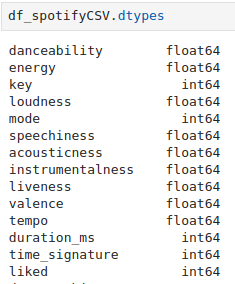
\includegraphics[width=.4\linewidth]{Draft Pipeline/pandas/Spotify-DTypes.png}
    \caption{The data types of the Spotify Likes Dataset.}
    \label{fig:Spotify-DTypes}
\end{figure}

\begin{figure}[H]
    \centering
    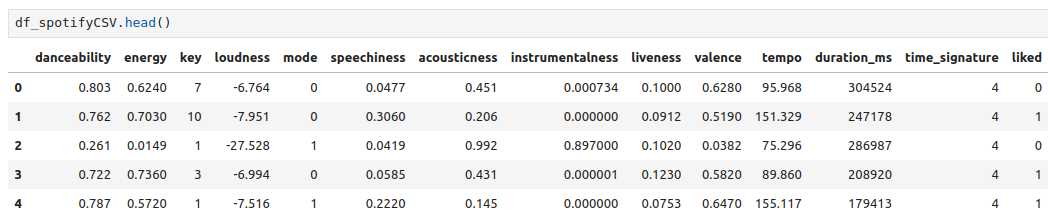
\includegraphics[width=\linewidth]{Draft Pipeline/pandas/Spotify-Head.png}
    \caption{The head of the dataset.}
    \label{fig:Spotify-Head}
\end{figure}

\begin{figure}[H]
    \centering
    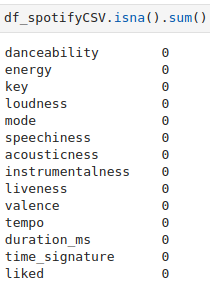
\includegraphics[width=.4\linewidth]{Draft Pipeline/pandas/Spotify-NA.png}
    \caption{No missing values in the dataset.}
    \label{fig:Spotify-NA}
\end{figure}

While a machine learning model to solve a binary classification problem could be trained on this dataset to identify if the author would like a song, 
it has significantly less of a positive impact than Candidates 1 and 3, as this dataset is the author's subjective belief rather than objective
fact that can be applied to other people. Nevertheless, the descriptions of each column can be found in Table \ref{tab:Spotify-Types}.

\begin{table}[H]
    \centering
    \begin{tabular}{ |p{0.2\textwidth}| p{0.45\textwidth}| p{0.2\textwidth}|}
        \hline
        \cellcolor{blue!25}Column & \cellcolor{blue!25}Description & \cellcolor{blue!25}Measurement level\\
            \hline
            Danceability & How suitable a song is for dancing measured from 0.0 to 1.0.
            & Ratio \\
            \hline
            Energy & The intensity and activity of a song. For example, death metal is high energy, whereas classical music is low intensity. 1.0 is the most energetic.
            & Ratio\\
            \hline
            Key & The musical key the song is in, converted to an integer using \href{https://smbutterfield.github.io/ibmt17-18/22-intro-to-non-diatonic-materials/b2-tx-pcintnotation.html}{standard pitch class notation.}\autocite{butterfield_22b_nodate} 
            & Ratio\\
            \hline
            Loudness & The averaged decibel volume of a song, typically between -60 and 0 dB.
            & Interval\\
            \hline
            Mode & Whether a song is in major or minor scale. 1 is major and 0 is minor.
            & Nominal\\
            \hline
            Speechiness & The calculated presence of spoken words in a song.
            & Ratio\\
            \hline
            Acousticness & A confidence measure from 0.0 to 1.0 of whether the track is acoustic. 1.0 represents high confidence the track is acoustic.
            & Ratio\\
            \hline
            Instrumentalness & A confidence measure from 0.0 to 1.0 of whether a song has no vocals.
            & Ratio\\
            \hline
            Liveness & A confidence measure from 0.0 to 1.0 of whether a live audience can be heard as part of a song.
            & Ratio\\
            \hline
            Valence & A confidence measure from 0.0 to 1.0 of the musical positiveness of a song.
            & Ratio\\
            \hline
            Tempo & The beats per minute of a song.
            & Ratio\\
            \hline
            Duration\_MS & The duration of a song in milliseconds.
            & Ratio\\
            \hline
            Time signature & The estimated time signature of the song.
            & Ratio\\
            \hline
            \cellcolor{red!15}Liked & The target variable, indicative of whether the author liked the song or not.
            & Ratio\\
            \hline
            \cellcolor{green!15}Type & Always "audio\_features". Not a relevant predictor.
            & Nominal\\
            \hline
            \cellcolor{green!15}ID & Spotify's own unique ID for a song. Not a relevant predictor.
            & Nominal\\
            \hline
            \cellcolor{green!15}URI & Spotify's URI for the song. Not a relevant predictor.
            & Nominal\\
            \hline
            \cellcolor{green!15}Track HREF & A link to the song on Spotify's API. Not a relevant predictor.
            & Nominal\\  
            \hline
            \cellcolor{green!15}Analysis URL & A link to the song's audio analysis data. Not a relevant predictor. 
            & Nominal\\
            \hline
    \end{tabular}
    \caption{The descriptions of each column in the Spotify songs dataset \autocite{spotify_web_nodate}. Red columns are only present in the CSV, whereas green columns are only present in the JSONs.}\label{tab:Spotify-Types}
\end{table}

These measurements and their descriptions are \href{https://developer.spotify.com/documentation/web-api/reference/get-audio-features}{sourced from Spotify's API},
and are automatically calculated when songs are uploaded to the service. The ground truth of the dataset is present in the CSV file as the "liked" classifier 
column, and a train/test split can be implemented for predictions, which is aided by the fact that this dataset is well balanced (100 liked to 95 disliked).
However, its small size and the fact that the model would only be able to predict one person's specific music taste make 
this dataset a poor candidate. 


\section{Candidate 3 - Loan Approval Classification Dataset}\label{sec:Dataset}
This dataset \autocite{lo_loan_nodate}, similarly to Candidate 2, was sourced from Kaggle's cloud servers under 
an Apache 2.0 license, which states that the dataset can be used as long as credit is given to the original author.
The dataset the physical form of a flat-file CSV, with the logical structure being the One Big Table data 
schema. 

\begin{figure}[H]
    \centering
    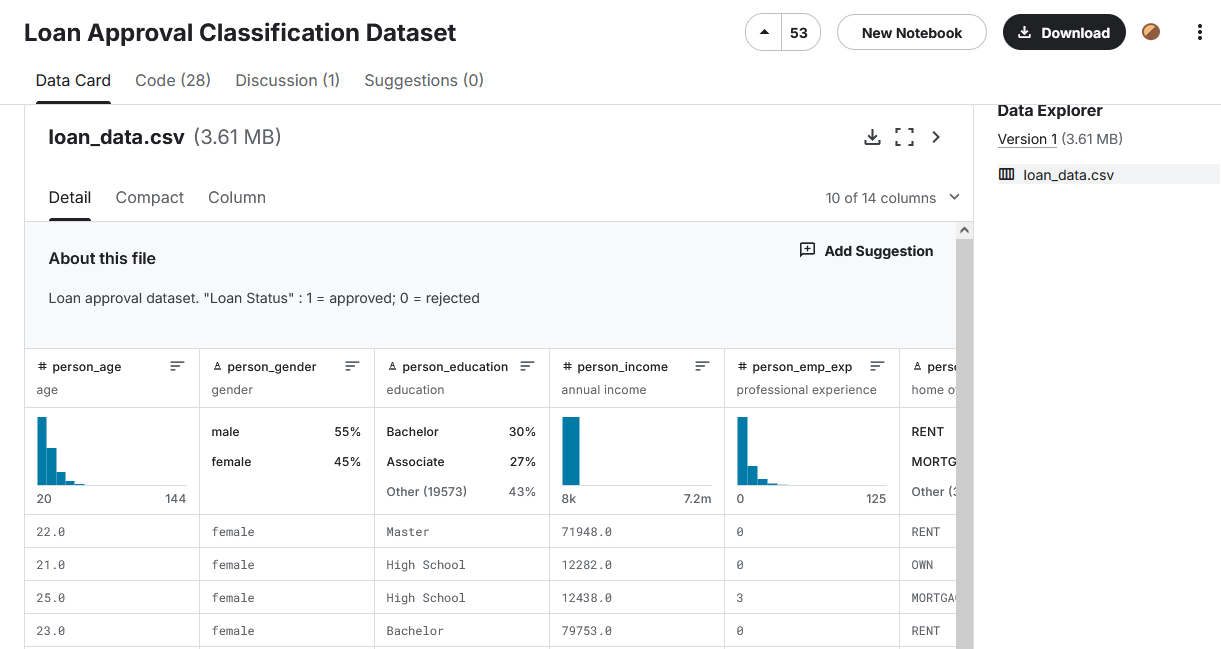
\includegraphics[width=.75\linewidth]{Draft Pipeline/Loan-Kaggle.png}
    \caption{A snapshot of the Loan dataset's Kaggle page.}
    \label{fig:Loan-Kaggle}
\end{figure}

Unlike Candidates 1 and 2, this dataset does not consist of real data, and 
instead consists of synthetic data. This is likely due to the fact that this dataset, if it used real data, would contain extremely personal 
information that could not be shared online due to legislation such as GDPR, which is further discussed in Section \ref{sec:dataTerms}. This particular dataset is an enhanced version of \href{https://www.kaggle.com/datasets/laotse/credit-risk-dataset}{a different credit risk dataset},
which also did not provide an original source and is also presumably synthetic data. The enhancements added were three additional 
columns, for the hypothetical person's gender, education level and credit score. Additionally, the author balanced the dataset using 
Synthetic Minority Oversampling Technique (SMOTE), an oversampling algorithm designed to balance datasets to produce higher
quality machine learning models \autocite{microsoft_smote_2024}.
It can therefore be established that this dataset was created solely for research and analysis purposes, including 
for the creation of supervised learning models. The dataset consists of 45,000 records and 14 features, with 
one of these being the ground truth target variable "loan\_status", which is whether the person should be given a loan or not. 
31 notebooks on Kaggle created by the site's users utilise this dataset, with many of these choosing to solve the binary classification 
problem that it presents, including works published by authors such as \autocite{gupta_loanification_2021}. 
The dataset is physically stored as a flat-file CSV, under a One Big Table (OBT) logical data schema.
The data types for each column can be seen in the entity relationship diagram and Pandas code in Figures \ref{fig:Loan-ERD} and \ref{fig:ILPD-DTypes}, and 
descriptions of each column can be seen in Table \ref{tab:Loan-Types}.

\begin{figure}[H]
    \centering
    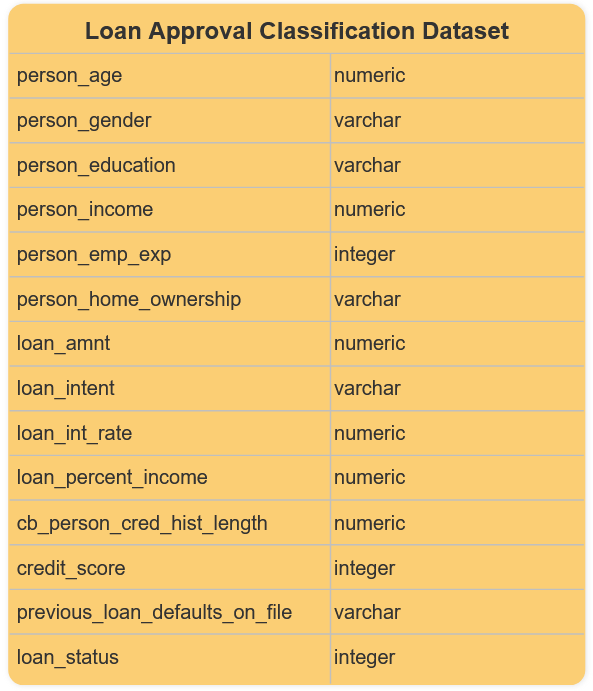
\includegraphics[width=.75\linewidth]{Draft Pipeline/Loan-ERD.png}
    \caption{An entity relationship diagram of the Loan Approval Classification Dataset.}
    \label{fig:Loan-ERD}
\end{figure}

\begin{figure}[H]
    \centering
    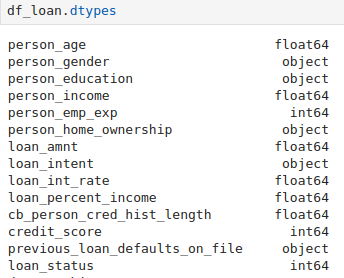
\includegraphics[width=.6\linewidth]{Draft Pipeline/pandas/Loan-DTypes.png}
    \caption{The data types of the Loan Approval Classification Dataset.}
    \label{fig:Loan-DTypes}
\end{figure}

\begin{figure}[H]
    \centering
    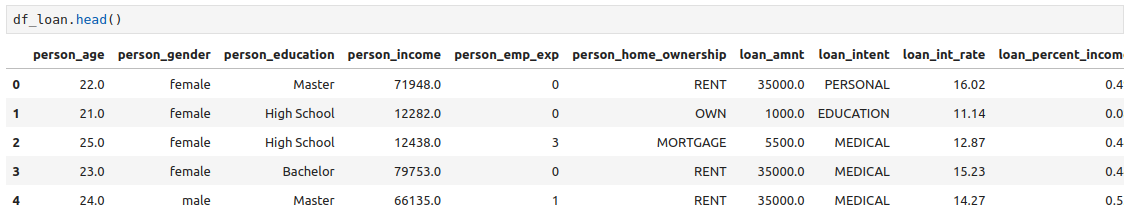
\includegraphics[width=\linewidth]{Draft Pipeline/pandas/Loan-Head.png}
    \caption{The head of the dataset.}
    \label{fig:Loan-Head}
\end{figure}

\begin{figure}[H]
    \centering
    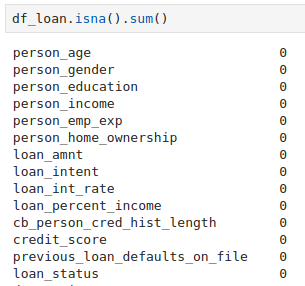
\includegraphics[width=.7\linewidth]{Draft Pipeline/pandas/Loan-NA.png}
    \caption{No missing values in the dataset.}
    \label{fig:Loan-NAs}
\end{figure}


\begin{table}[H]
    \centering
    \begin{tabular}{|p{0.4\textwidth}| p{0.4\textwidth}| p{0.15\textwidth} |}
        \hline
        \cellcolor{blue!25}Column & \cellcolor{blue!25}Description & \cellcolor{blue!25}Measurement level\\
            \hline
            person\_age & The age of the person. & Ratio\\
            \hline
            person\_gender & The person's gender. & Nominal\\
            \hline
            person\_education & The person's highest level of education. & Ordinal\\
            \hline
            person\_emp\_exp & The person's years of employment experience. & Ratio\\
            \hline
            person\_home\_ownership & Home ownership status (for example rent, own, mortgage)
            & Nominal\\
            \hline
            loan\_amnt & The amount of money requested. & Ratio\\
            \hline
            loan\_intent & The purpose of the loan. & Nominal\\
            \hline
            loan\_int\_rate & The interest rate of the loan. & Ratio\\
            \hline
            loan\_percent\_income & Loan amount as a percentage of the person's yearly income.
            & Ratio\\
            \hline
            cb\_person\_cred\_hist\_length & Length of credit history in years. & Ratio\\
            \hline
            credit\_score & Credit score of the person. & Ratio\\
            \hline
            previous\_loan\_defaults\_on\_file & If the person has defaulted on a loan before.
            & Nominal \\
            \hline
            loan\_status & Whether the loan should be approved. 1 if yes, 0 if no.
            & Nominal\\
            \hline
    \end{tabular}
    \caption{The descriptions of each column in the dataset.}\label{tab:Loan-Types}
\end{table}

This dataset is also frequently updated, with its most recent update occurring on the 29th of October.
This would mean it may be more suited to an OLTP database system, which will be further discussed in Section 
\ref{sec:Ingestion}.

\section{Chosen dataset}
Of the three candidates presented, the most suitable for a machine learning operations pipeline would be Candidate 3, the loan approval dataset. As mentioned 
in Section \ref{sec:Dataset}, this dataset possesses many predictor variables and an adequate amount of data to train a supervised learning classification model 
to classify whether an individual should be allowed a loan or not. While the data in this dataset is synthetic due to its real equivalent being highly protected 
under data protection legislation, the model trained from said synthetic data could be applied to real data using what it has learned, and could greatly expedite 
the process of loan approvals.

As previously mentioned, the dataset is hosted on Kaggle's cloud database, in the physical structure of a  
CSV file, using a One Big Table (OBT) data schema for its logical structure.  
Libraries such as Pandas natively work with these types of files which will allow for quick ingestion. 
When the dataset is ingested, it will be stored in a MariaDB Columnstore instance, which is further 
described in Section \ref{ch:PlanMLOps}. For this pipeline, the data will be kept in the OBT schema
due to the simplicity and efficiency of queries performed on it, and also to ensure maximum data integrity
that could be lost if the logical structure were modified. There were other options that could have been used
instead of OBT, represented in Table \ref{tab:Schemas}


\begin{longtable}{ |p{0.15\textwidth}| p{0.22\textwidth}| p{0.2\textwidth} | p{0.25\textwidth} | }
    \hline
    \cellcolor{blue!25}Schema & \cellcolor{blue!25}Description & \cellcolor{blue!25}Positives & \cellcolor{blue!25}Negatives \\
    \hline
    Star
    \autocite{kaminsky_star_nodate} & Stores data across a main fact table for measured or transactional data, and dimension tables 
    for data related to the fact data, which can be visualised like a star. & Simple to understand, few joins needed,
    very scalable. & Data updates would require updates of multiple rows in multiple tables. Adding new columns
    (dimensions) after initial creation can be difficult because the schema is denormalised.\\
    \hline
    Snowflake
    \autocite{geeksforgeeks_snowflake_2023} & An extended form of the Star schema that further branches its dimension tables
    into a hierarchy, appearing more like a snowflake than a star due to the multiple branches formed. &
    Unlike a star schema, data is normalised, allowing data to be added easier than a star schema. & More 
    complex to query due to the increased amount of tables, therefore requiring more processing power. \\
    \hline
    Normalised Relational Model 
    \autocite{microsoft_database_2024} & Heavily organises data, and emphasises the relationships between tables. &
    Keeps minimal or no redundant data whatsoever, reducing storage requirements. In doing so, this also heightens 
    data integrity. & As with other schemas that use many tables, queries can be slowed by the need for multiple 
    joins. \\
    \hline 
    \caption{An analysis of alternative data schemas.}\label{tab:Schemas}
\end{longtable}


\chapter{Planning the MLOps Pipeline}\label{ch:PlanMLOps}
All machine learning operations (MLOps) follow a five-step repeatable pipeline, outlined in Figure \ref{fig:MLPipeline}, where the output of one stage
becomes the input of the next. 
\begin{figure}[H]
    \centering
    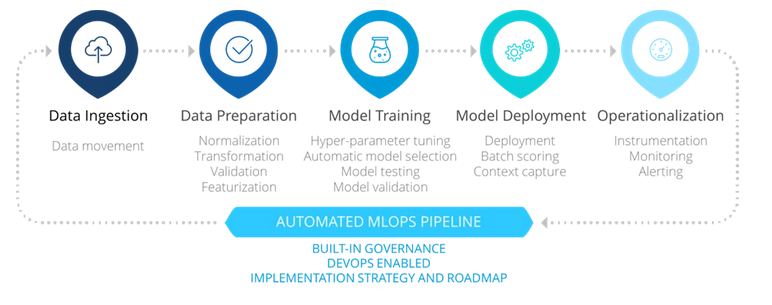
\includegraphics[width=.75\linewidth]{Draft Pipeline/MLPipeline.png}
    \caption{The five key steps in an MLOps pipeline \autocite{incycle_software_mlops_nodate}.}
    \label{fig:MLPipeline}
\end{figure}
The pipeline begins with raw data and finishes with a trained machine learning model, and is often 
repeated at certain intervals, which could be as simple as once a day, or it could be repeated as new data becomes available. 
This repetition is performed automatically, so that the final model can become progressively more accurate. Because the process 
must be repeatable and automated, it is essential that data is validated to ensure that one run of the pipeline where the data may have 
been corrupted somehow would not cause issues, which would quickly spiral out of control as the pipeline is repeated again and again.
Overall, MLOps pipelines standardise the development and deployment process of machine learning models, ensuring continuous integration
(CI) and continuous delivery (CD) and enhancing collaboration between data scientists and development teams.

\pagebreak

\section{Software to be used in the pipeline}
A wide variety of software will be used across the MLOps pipeline, with an overall glossary of them documented in Table \ref{tab:softwareDescriptions}.
Descriptions on how they will specifically be used in each stage of the pipeline can be found in each stage's respective
section.

\begin{longtable}{ |p{0.2\textwidth}| p{0.8\textwidth}|}
    \hline
    \cellcolor{blue!25}Software/Library & \cellcolor{blue!25}Overview\\
    \hline
    Conda 
    & A package and environment management system which allows 
    for software developers and data scientists to easily control the libraries used in their code \autocite{anaconda_about_nodate}. 
    Allows for the creation of \textbf{virtual environments}, which are contained structures where packages can be installed.
    The use of virtual environments allows for specific versions of packages to be kept, for instance with one environment 
    storing an older version of a library for compatibility purposes, with another storing a newer version to be used in a different project. 
    Were it not for these virtual environments, developers would constantly have to uninstall and reinstall specific package versions, wasting 
    considerable amounts of time. Conda also hosts its own repositories to obtain packages from, and a 
    major benefit of Conda occurs during the package installation process, which is that it will identify 
    dependencies and version clashes between packages and solve them automatically, once again saving 
    considerable amounts of time.
    
    In this project, Conda will be used as the environment and package manager to install and contain the 
    libraries used in the development process. To do so, the Miniconda distribution will be installed, as 
    this is a smaller distribution to save hard disk space and download time, but still contains the key 
    Conda backend, as seen in Figure \ref{fig:Miniconda}. \\
    \hline
    Apache Airflow &
    A platform used to orchestrate workflows and pipelines entirely in Python code \autocite{apache_use_nodate}.
    Airflow creates Directed Acyclic Graphs (DAGs), which map out the order and dependencies of each task in a 
    pipeline, and runs tasks in the order specified within the DAG, while also accounting for dependencies.
    Also provides many useful features such as task scheduling, which is especially useful for the automation 
    of an MLOps pipeline, as well as automatic failure handling, where actions can automatically be performed 
    on a task's failure, such as stopping the pipeline to prevent wasting computational resources. Airflow 
    also provides a convenient UI, accessible by using the command "airflow webserver", which will host a 
    web UI where tasks can be run, paused or stopped, as well as viewed in a tree view that maps the 
    sequence and dependencies of tasks. Airflow also provides "Operators", which handle running code such 
    as Python and Bash scripts.

    Airflow will be used within this project at all stages of the pipeline in order to manage the overall 
    execution and structure of tasks. Operators will be used for the execution of all Python or Bash 
    commands throughout the pipeline. By using Airflow in this way, the pipeline can become completely 
    automated with continuous integration and continuous deployment.
    \\
    \hline
    Docker &
    An open-source containerisation system used to enhance the portability of applications by distributing 
    them as self-contained, lightweight instances that come with everything they need to run immediately 
    without needing to worry about system incompatibility (\textcite{aws_what_nodate}, \textcite{docker_docker_2022})
    and minimise issues where software can run on one computer but not another. Docker could be described 
    as working similarly to a virtual machine, though it is considerably more lightweight as it is not 
    virtualising hardware.\\
    \hline
    MariaDB Columnstore &
    A columnar storage engine designed for the processing of petabytes of data with high performance 
    and real-time response regardless of dataset size \autocite{mariadb_mariadb_nodate}. While 
    primarily intended for OLAP databases, it also facilitates OLTP databases. A Docker container 
    for this software will be used in this pipeline.\\
    \hline 
    Redis &
    An in-memory data store used to cache data in a machine's RAM rather than its 
    persistent storage. The benefits of this are that said data can be loaded many times faster than if 
    it were loaded from a hard drive. This does therefore mean that Redis will not be used to store persistent data,
    and it will instead be used to transfer data between different tasks in an Airflow DAG, as Airflow tasks 
    are independent from each other. Redis will solve this by having relevant data loaded into memory before 
    the task ends, at which point it will be read by the following task. A Docker container for this 
    software will be used in this pipeline. Also includes a Python library of the same name that allows 
    for access to the Redis store from Python scripts.\\
    \hline
    Pandas &
    A library used widely in industry for data analytics. It is capable of importing data of various 
    types and storing them in a "DataFrame" object, which preprocessing operations can be performed on.
    It also allows the exporting of data in multiple formats \autocite{pandas_pandas_nodate}.\\
    \hline
    SQLAlchemy &
    A library that allows SQL engine connections to be made from within a Python file. In 
    doing so, data can be read from and stored into SQL databases \autocite{sqlalchemy_sqlalchemy_nodate}.\\
    \hline
    Scikit-learn & 
    A large open-source Python library containing many different functionalities for machine learning \autocite{scikit-learn_scikit-learn_nodate}, 
    such as encoders to convert strings to numerical equivalents, scalers to normalise and standardise 
    the data to reduce variance (described further in Section \ref{sec:Preprocessing}), as well as containing 
    methods to split data into training and testing sets, and fit, train and predict with various different 
    machine learning algorithms (described further in Section \ref{sec:Development}).\\
    \hline
    FastAPI &
    A high-performance framework for developing APIs in Python, proclaimed
    as "One of the fastest Python frameworks available" \autocite{fastapi_fastapi_nodate}.
    Facilitates an API for clients to access the backend ML model later in the pipeline. \\
    \hline
    Uvicorn &
    A low-level webserver implementation in Python with high performance \autocite{uvicorn_uvicorn_nodate}.\\
    \hline
    MLFlow &
    An open-source platform for the tracking and monitoring of machine learning models, 
    storing each iteration of the model so that they may be reproduced at a later point \autocite{mlflow_mlflow_nodate},
    which is especially useful while performing hyperparameter tuning on the model, which is where 
    small details of the model are changed such as the number of decision trees in a Random Forest.
    Also facilitates REST APIs, discussed in Section \ref{sec:Deployment}.\\
    \hline
    Apache Arrow \newline PyArrow &
    Software with a Python library interface that allows for the serialization of objects \autocite{apache_streaming_nodate}. 
    This is important in synergy with Redis and Pandas, as Redis is unable to directly store Pandas dataframes, 
    so they must first be serialized, converting them to a bytes format that Redis can store in memory.\\
    \hline
    Pickle &
    A base package in Python that functions similarly to Arrow in the serialization of data \autocite{python_pickle_nodate}.
    Pickle specifically will be used to serialize machine learning models.\\
    \hline
    Great Expectations &
    A Python library used for data validation, where "expectations" can be set for a dataset, such as 
    all data of a column being numeric, and they will be assessed \autocite{gx_gx_nodate}.\\
    \hline
\caption{Descriptions of software and libraries across the pipeline.}\label{tab:softwareDescriptions}
\end{longtable}

\begin{figure}[H]
    \centering
    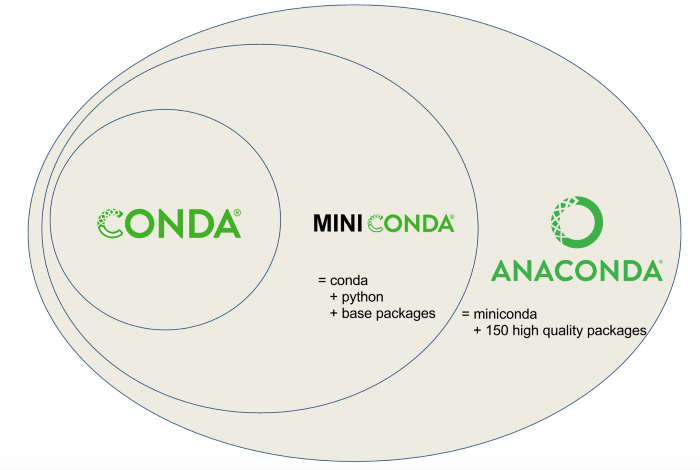
\includegraphics[width=.75\linewidth]{miniconda.png}
    \caption{A comparison of the primary Conda distributions \autocite{towardsdatascience_getting_2021}}
    \label{fig:Miniconda}
\end{figure}

\pagebreak

\section{Data Ingestion}\label{sec:Ingestion}
% \subsubsection{Input: Raw Data from Original Source (Loan CSV from Kaggle)\\Output: Ingested Data (Data in MariaDB Columnstore)}
\subsection{Description}
The first step of any machine learning pipeline is data ingestion. This refers to the process of obtaining the input data from its original source
and transferring it to a relevant storage medium, such as a database or data warehouse, to be used in later stages. This stage 
is undertaken by data scientists. 
It is of vital importance that data is not lost or corrupted during ingestion, as this stage is the baseline for all future stages in the pipeline, and any issues
here will directly impact all future stages, as previously discussed. Furthermore, when ingesting data, it is important to understand what type of system this data 
will be used in, of which there are two options: Online Analytics Processing Systems (OLAP), and Online Transactional Processing Systems (OLTP), as well 
as how it will be loaded into the chosen system, either using an ELT (Extract, Load, Transform) or ETL (Extract, Transform, Load) methodology.

\subsubsection{OLAP and OLTP}

\begin{table}[H]
    \centering
        \begin{tabular}{ |p{0.4\textwidth}| p{0.425\textwidth}|}
            \hline
            \cellcolor{blue!25}OLAP & \cellcolor{blue!25}OLTP\\
            \hline
            Designed for complex queries and data analysis, primarily data reading.
            & Designed for lots of short, fast queries ("transactions") for both reading and writing.\\
            \hline
            Typically store massive amounts of data, sometimes petabytes.
            for extremely detailed analysis. 
            & Usually store less data for speed purposes.\\
            \hline
            Usually historical data, infrequently updated. 
            & Typically real-time data that is updated often.\\
            \hline 
            Uses database schemas such as star or snowflake schema to allow for queries using many joins. 
            & Uses normalised or denormalised models, such as One Big Table, minimising joins and maximising speed.\\
            \hline
            Slow response times, measured in minutes. 
            & Fast response times, measured in milliseconds.\\
            \hline
    \end{tabular}
    \caption{A comparison of OLAP and OLTP systems \autocite{aws_oltp_nodate}.}\label{tab:OLAP-OLTP}
\end{table}

As mentioned in Table \ref{tab:OLAP-OLTP}, OLAP systems are designed for complex and deep data analytics, which helps 
companies perform tasks such as analysing customer trends, while OLTP systems aim for maximum speed to complete quick transactions, 
which is necessary in situations like processing payments and orders.

\subsubsection{ELT and ETL}
ELT and ETL are both acronyms for the order of processes taken when ingesting data, with "Transform" either 
happening before or after the data is loaded into a storage medium like a data warehouse or data lake. 
The extract phase refers to the initial gathering of the data from its original source, such as Kaggle for 
the selected dataset in this report. The transform phase refers to early modifications made to the data, such 
as formatting or cleaning, and the load phase refers to the transportation of the data from its original storage
medium (a CSV on Kaggle's cloud servers in this case) to a more optimised and efficient data warehouse to be used 
in the execution of the pipeline.

Regardless of whether ETL or ELT is used, the data is still extracted, loaded and transformed. However,
the decision of which order to use can be determined from the data itself, with smaller datasets that may need 
complex transformation from their raw form being more suited to ETL, whereas large datasets with less 
transformation needed can be better with ELT \autocite{smallcombe_etl_nodate}.

\begin{table}[H]
    \centering
        \begin{tabular}{ |p{0.4\textwidth}| p{0.425\textwidth}|}
            \hline
            \cellcolor{blue!25}ELT & \cellcolor{blue!25}ETL\\
            \hline
            Data is transformed \textbf{after} being loaded into another storage medium.
            & Data is transformed \textbf{before} being loaded into another storage medium. \\
            \hline
            Useful if the data warehouse is a more modern system with good processing power.
            & Useful if the data warehouse has limited processing abilities of its own,
            typically seen in older or otherwise less powerful systems such as those on 
            virtual machines.\\
            \hline
            Lower latency in the ingestion phase because data is immediately loaded. 
            & Higher latency in the ingestion phase, because the data is being processed first, 
            adding an extra time overhead where the pipeline could be held up.\\
            \hline 
            Simpler to set up due to the immediate loading of the data.
            & Can be complex to set up and maintain, as the transformation would occur outside the warehouse.\\
            \hline
    \end{tabular}
    \caption{A comparison of ETL and ELT methodologies (\textcite{bartley_etl_2024}, \textcite{aws_etl_nodate}).}\label{tab:ELT-ETL}
\end{table}

It can be surmised from the analysis of each method in Table \ref{tab:ELT-ETL} that ETL is best applied 
to older systems with limited processing power, whereas ELT is better in more modern systems. 
It can additionally be argued that performing the ETL order of operations blurs the line between the ingestion and 
preprocessing stages, as the data is transformed before it is actually loaded into the system and
fully ingested, whereas ELT has a clear split between the ingestion and preprocessing of the data. 

\subsection{In this project}
The candidate dataset's raw CSV file, downloaded directly from Kaggle, will act as the input for this stage. It utilises the One Big Table schema, 
and it was previously established in Section \ref{sec:Dataset} that it contains no missing values. 
The size of the dataset is the largest of the three candidates but is still
small in comparison to those used in industry, being only 3.5MB in comparison to gigabytes and petabytes as previously 
mentioned in Table \ref{tab:OLAP-OLTP}. Because of this small size, processing operations performed on the dataset 
will be very fast, even with limited processing power, so the ETL methodology will be used to ingest the data 
into a MariaDB Columnstore OLTP database for quick and efficient loading and querying, where the end user will be 
able to quickly supply predictor variables and receive a fast response. To do so, 
some of the software originally mentioned in Table \ref{tab:softwareDescriptions} will be used, seen in Table \ref{tab:IngestionSoftware}.




\begin{longtable}{ |p{0.2\textwidth}| p{0.5\textwidth}|}
    \hline
    \cellcolor{blue!25}Software/Library & \cellcolor{blue!25}Usage for ingestion\\
    \hline
    Docker &
    In this stage, Docker will be used to host a container of MariaDB Columnstore.\\
    \hline
    MariaDB Columnstore &
    In this stage, the Columnstore will be hosted on a Docker container at port 3306 \autocite{docker_hub_mariadbcolumnstore_nodate}, 
    and will be used as the OLTP storage medium of the ingested data.\\
    \hline 
    Pandas &
    In the ingestion phase, it will be used to import the dataset's CSV file, and export it as SQL to 
    the MariaDB Columnstore through the use of SQLAlchemy.\\
    \hline
    SQLAlchemy &
    Alongside Pandas, SQLAlchemy will export the DataFrame to the MariaDB Columnstore instance.\\
    \hline
\caption{Software to be used in ingestion.}\label{tab:IngestionSoftware}
\end{longtable}

\begin{figure}[H]
    \centering
    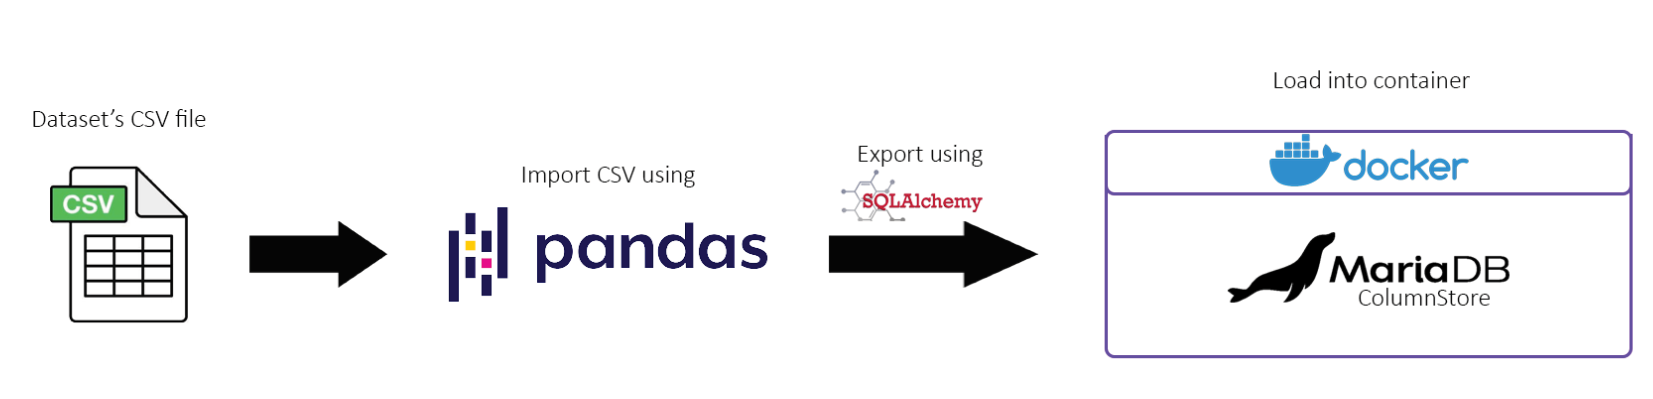
\includegraphics[width=.9\linewidth]{diagrams/Ingestion.png}
    \caption{A diagram of the planned ingestion process.}
    \label{fig:IngestionDiagram}
\end{figure}

\pagebreak % separating Fig 2.3 from preprocessing section.

\section{Data Preprocessing}\label{sec:Preprocessing}
\subsection{Description}
After the data has been ingested, the preprocessing stage begins, and is often also conducted by 
Data Scientists. This stage encompasses the
cleaning, integration and transformation of the data in order to optimise the dataset for model development.

Cleaning refers to the identification of missing, inaccurate or malformed data within the dataset,
as well as its removal or imputation where possible.

Integration is often seen in datasets with multiple tables or that have been retrieved from multiple sources,
and refers to the combination of the retrieved data into a single flat file. 

Transformation, also known as feature engineering, is a considerable aspect of data preprocessing
which refers to the manipulation and formatting of the data, such as changing the formats of columns 
from numeric dates to proper date data types, as well as the handling of categorical data, such as genders, 
which may originally be strings. Strings cannot be interpreted by machine learning models, and therefore they 
are encoded into numbers using techniques such as label encoding, which converts the unique values in a column
to a numerical representation, such as male being 0 and female being 1. Data is also normalised and standardised 
in this stage, meaning that numerical data is reduced to being between 0 and 1 to adjust the overall scale of the 
data. This is especially useful with algorithms such as K-Nearest Neighbours, where large differences in distance 
between data can mislead the classification algorithm \autocite{ibm_what_2021}.

Once these tasks have all been completed, the dataset will be ready to be used for model development.

\subsection{In this project}
The preprocessing in this project will take the ingested data as input, from which point it will be transformed,
with columns such as "person\_gender" encoded to categorically labelled numerical equivalents. To do so, some of the software
and libraries originally mentioned in Table \ref{tab:softwareDescriptions} will be used, shown below in Table \ref{tab:PreprocessingSoftware}.
After this, the processed dataset will be output to Redis, to be used as the input for the model development stage.


\begin{longtable}{ |p{0.2\textwidth}| p{0.5\textwidth}|}
    \hline
    \cellcolor{blue!25}Software/Library & \cellcolor{blue!25}Usage for preprocessing\\
    \hline
    Pandas & 
    Will be used alongside SQLAlchemy to load the dataset from the MariaDB Columnstore instance hosted on Docker, 
    as well as for the actual transformation of the data using the methods provided by Pandas dataframes.\\
    \hline
    SQLAlchemy & 
    Will be used alongside Pandas to query and receive data from the MariaDB Columnstore instance.\\
    \hline
    Scikit-learn & 
    Will be used to normalise and standardise the data, as well as encode any string data into numerical 
    equivalents.\\
    \hline
    Docker &
    Will host the MariaDB Columnstore container. Additionally for this section, it will also host a 
    container for Redis to store the processed dataset.\\
    \hline
    Redis &
    Will store the processed dataframe in memory. Cannot directly store the dataframe as mentioned in 
    Table \ref{tab:softwareDescriptions}, so it must be serialised first using Arrow.\\
    \hline
    Arrow & 
    Will serialise the processed dataframe so that it can then be stored by Redis.\\
    \hline
\caption{Descriptions of software to be used for preprocessing.}\label{tab:PreprocessingSoftware}
\end{longtable}

\begin{figure}[H]
    \centering
    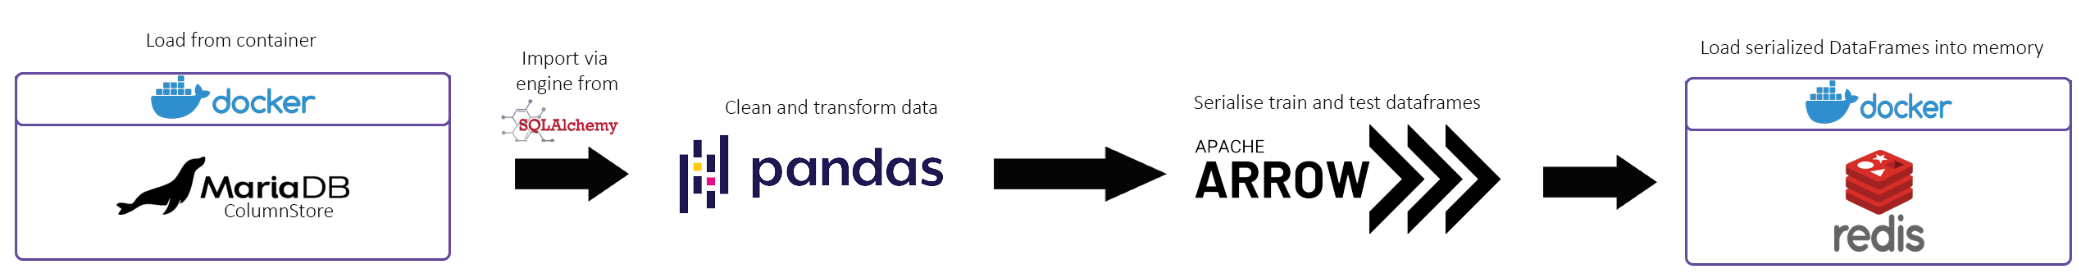
\includegraphics[width=.9\linewidth]{diagrams/Preprocessing.png}
    \caption{A diagram of the planned preprocessing stage.}
    \label{fig:PreprocessingDiagram}
\end{figure}


\pagebreak

\subsection{Data analysis} % Missed this from the original submission.
To build a machine learning model for a dataset, it greatly helps to understand the data itself.

\subsubsection{Distributions and outliers}
Understanding the data means to know how the data is typically distributed, and what constitutes an outlier. This can be 
done through visualisations such as box plots for numerical data and bar charts for categorical data.

\begin{figure}[H]
    \centering
    \begin{subfigure}[b]{0.3\textwidth}
        \centering
        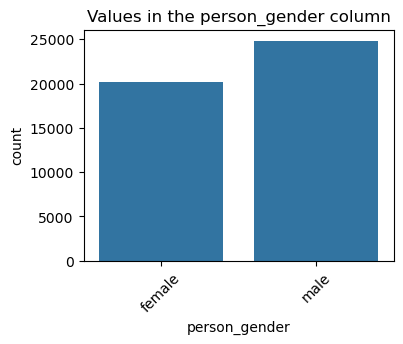
\includegraphics[width=\textwidth]{Plots/Gender.png}
        \caption{Genders}
        \label{fig:Bar1}
    \end{subfigure}
    \hfill
    \begin{subfigure}[b]{0.3\textwidth}
        \centering
        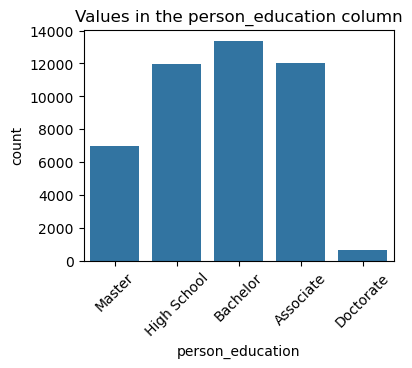
\includegraphics[width=\textwidth]{Plots/Education.png}
        \caption{Education levels}
        \label{fig:Bar2}
    \end{subfigure}
    \hfill
    \begin{subfigure}[b]{0.3\textwidth}
        \centering
        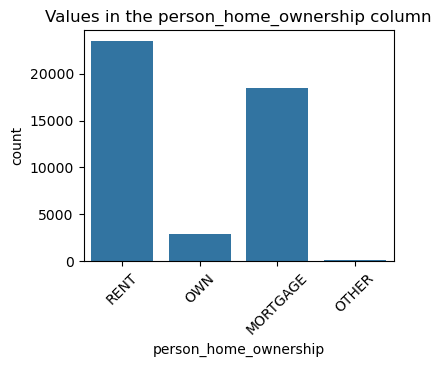
\includegraphics[width=\textwidth]{Plots/HomeOwnership.png}
        \caption{Home ownership}
        \label{fig:Bar3}
    \end{subfigure}
    
    \vspace{1em}
    
    \begin{subfigure}[b]{0.3\textwidth}
        \centering
        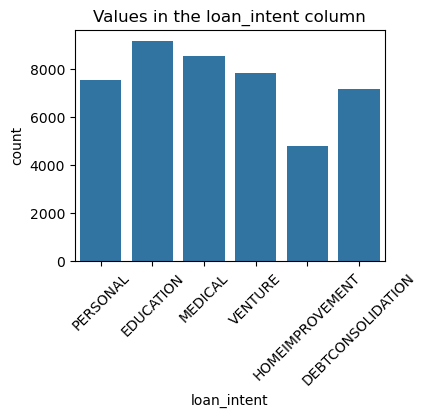
\includegraphics[width=\textwidth]{Plots/LoanIntent.png}
        \caption{Loan intents}
        \label{fig:Bar4}
    \end{subfigure}
    \hfill
    \begin{subfigure}[b]{0.3\textwidth}
        \centering
        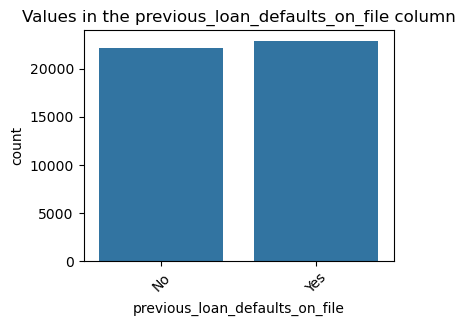
\includegraphics[width=\textwidth]{Plots/DefaultsOnFile.png}
        \caption{Previously defaulted}
        \label{fig:Bar5}
    \end{subfigure}
    \hfill
    \begin{subfigure}[b]{0.3\textwidth}
        \centering
        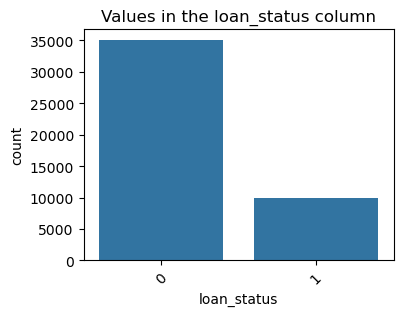
\includegraphics[width=\textwidth]{Plots/LoanStatus.png}
        \caption{Loan status}
        \label{fig:Bar6}
    \end{subfigure}
    \caption{Bar charts of the six categorical rows.}
    \label{fig:BarCharts}
\end{figure}

A notable observation is that the dataset is imbalanced, containing fewer records of granted 
loans than denied loans.

\begin{figure}[H]
    \centering
    \begin{subfigure}[b]{0.22\textwidth}
        \centering
        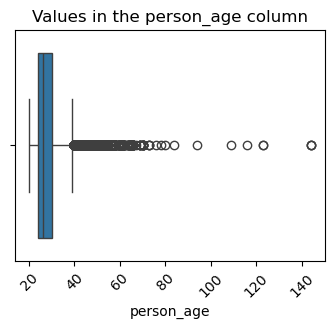
\includegraphics[width=\textwidth]{Plots/Age.png}
        \caption{Age}
        \label{fig:Boxplot1}
    \end{subfigure}
    \hfill
    \begin{subfigure}[b]{0.22\textwidth}
        \centering
        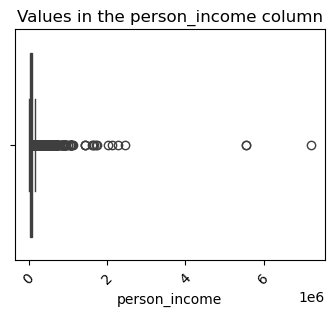
\includegraphics[width=\textwidth]{Plots/Income.png}
        \caption{Yearly income}
        \label{fig:Boxplot2}
    \end{subfigure}
    \hfill
    \begin{subfigure}[b]{0.22\textwidth}
        \centering
        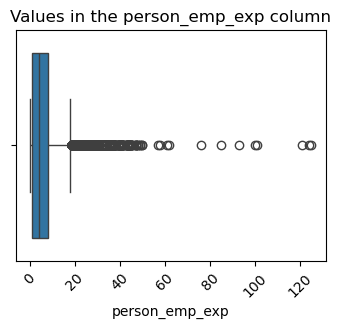
\includegraphics[width=\textwidth]{Plots/Employment.png}
        \caption{Previous jobs}
        \label{fig:Boxplot3}
    \end{subfigure}
    \hfill
    \begin{subfigure}[b]{0.22\textwidth}
        \centering
        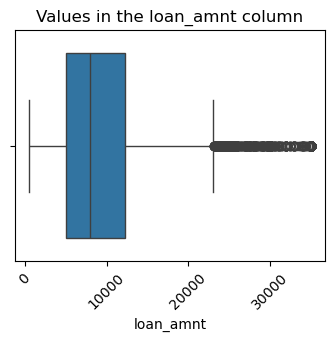
\includegraphics[width=\textwidth]{Plots/LoanAmount.png}
        \caption{Loan amount}
        \label{fig:Boxplot4}
    \end{subfigure}
    
    \vspace{1em}
    
    \begin{subfigure}[b]{0.3\textwidth}
        \centering
        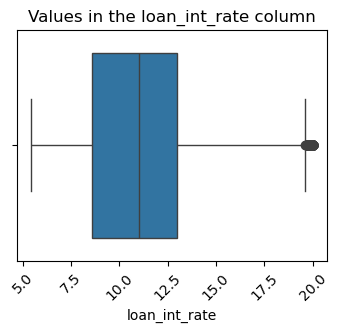
\includegraphics[width=\textwidth]{Plots/InterestRate.png}
        \caption{Interest rate}
        \label{fig:Boxplot5}
    \end{subfigure}
    \hfill
    \begin{subfigure}[b]{0.3\textwidth}
        \centering
        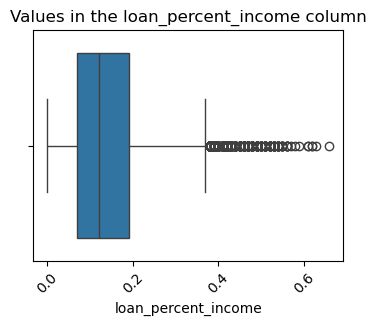
\includegraphics[width=\textwidth]{Plots/PercentIncome.png}
        \caption{Percentage of income}
        \label{fig:Boxplot6}
    \end{subfigure}
    \hfill
    \begin{subfigure}[b]{0.3\textwidth}
        \centering
        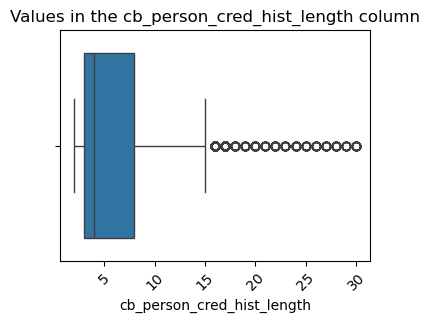
\includegraphics[width=\textwidth]{Plots/CreditHistory.png}
        \caption{Credit history length}
        \label{fig:Boxplot7}
    \end{subfigure}
    
    \caption{Box plots of all numerical columns.}
    \label{fig:Boxplots}
\end{figure}

There are many outliers in this dataset, most notably in the income column, where very few are earning millions.
Also, the age column has some outliers of extremely old people, including one aged 140, who cannot exist as the oldest 
person known was 112 before they died \autocite{sky_news_worlds_nodate}. This can therefore likely be attributed 
to erroneous generation due to this dataset being synthetic, and records with considerable outliers like this can 
be safely removed in the implementation's preprocessing phase.

\subsubsection{Encoding}
Machine learning models cannot directly interpret string data. Therefore, strings must be encoded to numerical representations
through either label encoding or one-hot encoding. Label encoding is best suited to ordinal data as it will maintain the ordering 
of said data, such as levels of education. One-hot encoding is better suited to nominal data without an inherent order, such as 
the intent of a loan. Therefore, this dataset requires the use of both types of encoding, shown in Figures \ref{fig:LabelEncoding}
and \ref{fig:OneHotEncoding}

\begin{figure}[H]
    \centering
    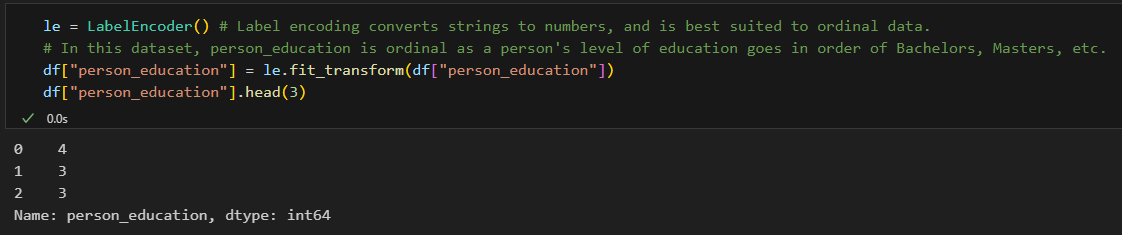
\includegraphics[width=\linewidth]{pandas/LabelEncoding.png}
    \caption{Using label encoding for the person\_education column.}
    \label{fig:LabelEncoding}
\end{figure}

\begin{figure}[H]
    \centering
    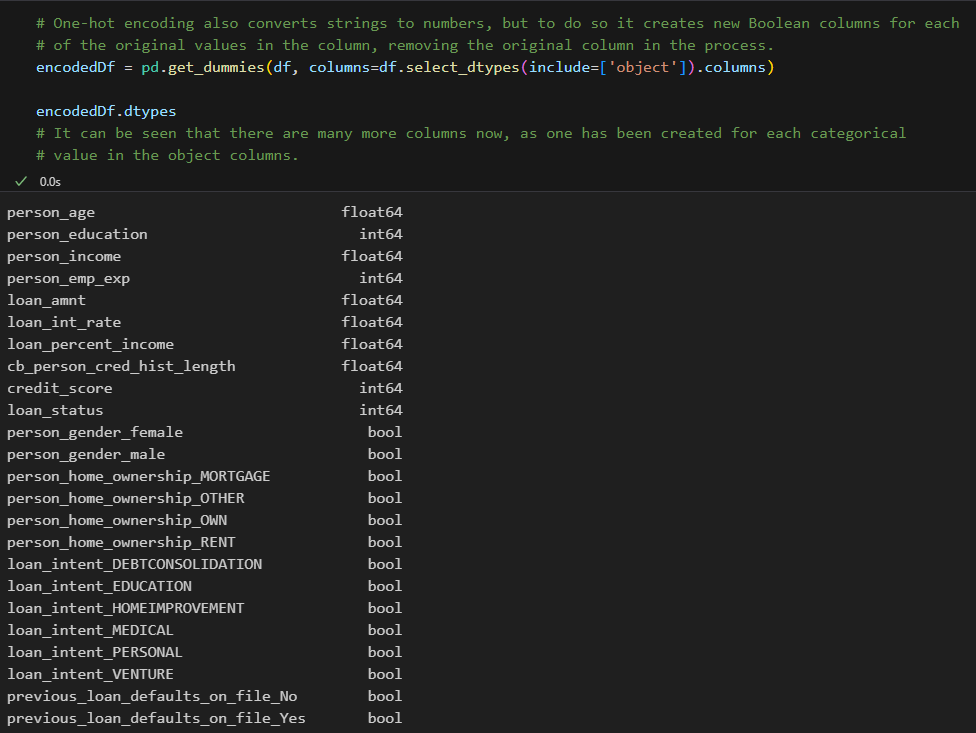
\includegraphics[width=\linewidth]{pandas/OneHotEncoding.png}
    \caption{Using one-hot encoding for the person\_education column.}
    \label{fig:OneHotEncoding}
\end{figure}

\subsubsection{Correlations}
The easiest way to view the correlations between variables is through a correlation matrix, seen below in Figure \ref{fig:BigMatrix}, which 
cannot be created unless data is first encoded. However, an immediate observation is the sheer size of the matrix due to an unfortunate side 
effect from one-hot encoding creating entirely new columns, increasing the dimensionality of the dataset. 

\begin{figure}[H]
    \centering
    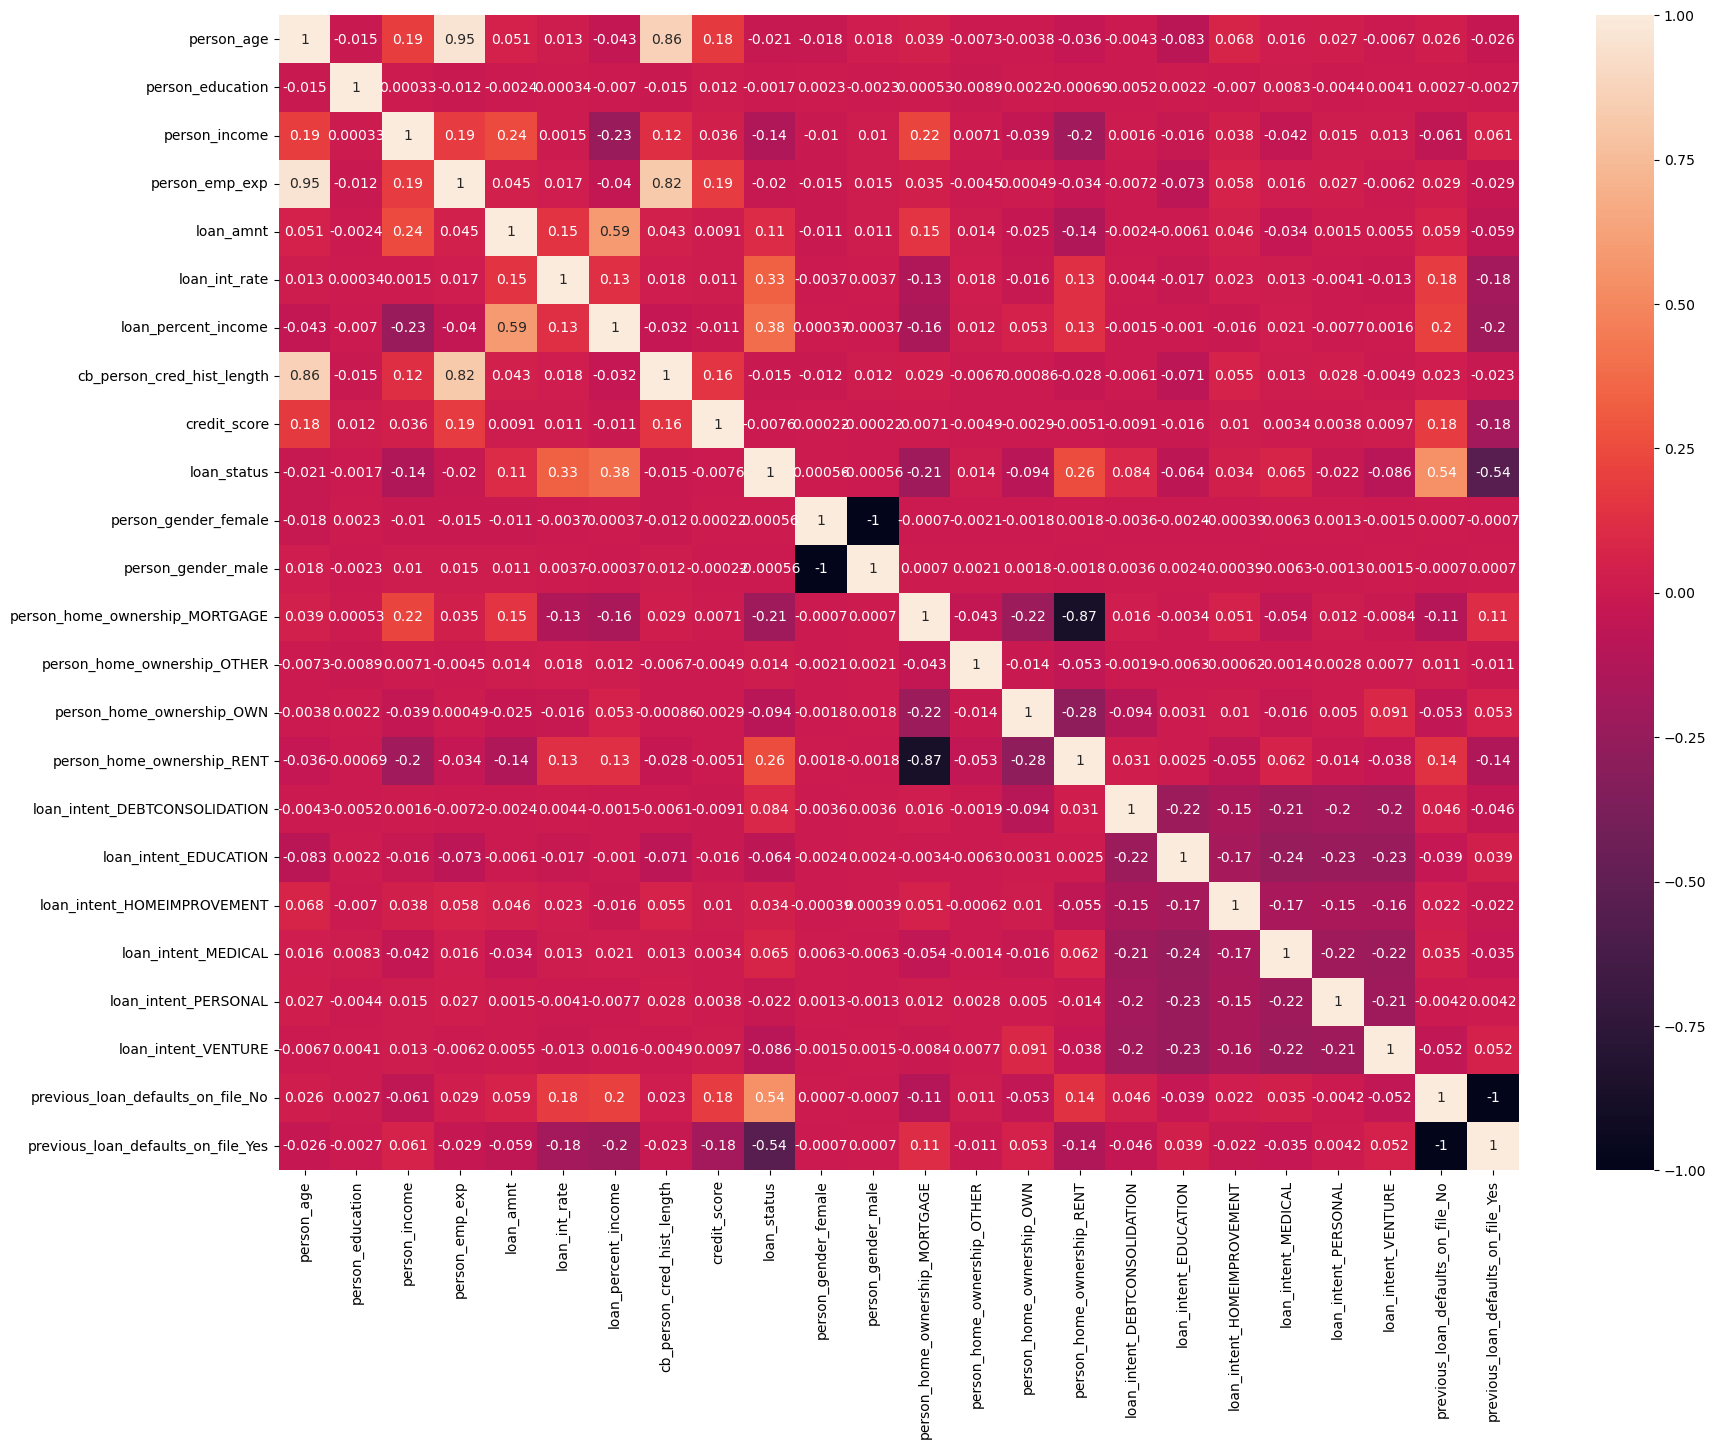
\includegraphics[width=\linewidth]{Plots/BigMatrix.png}
    \caption{The full correlation matrix for the encoded dataset.}
    \label{fig:BigMatrix}
\end{figure}

% To remedy this, the matrix can be produced after first filtering the dataset's correlations to only include rows with over 0.5 correlation 
% to each other. This is not a necessary process, but was done for easier viewing.

% \begin{figure}[H]
%     \centering
%     \includegraphics[width=\linewidth]{Plots/MiniMatrix.png}
%     \caption{The filtered correlation matrix for the encoded dataset.}
%     \label{fig:MiniMatrix}
% \end{figure}

Despite this, key insights can still be made about the likelihood of a loan being granted, such as:

\begin{itemize}
    \item Loans are most likely to be approved if the person has never defaulted on a loan before.
    \begin{itemize}
        \item They are least likely to be approved if the person has defaulted before.
    \end{itemize}
    \item The interest rate positively correlates with the loan's approval.
    \item If the person rents their home, they are more likely to be approved.
    \begin{itemize}
        \item They are less likely to be approved if they have a mortgage.
    \end{itemize}
    \item Loans are more likely to be approved if they are a large percentage of the person's yearly income.
\end{itemize}

\section{Model Development}\label{sec:Development}
\subsection{Description}
The model development stage accepts the processed dataset from the preprocessing stage as input and leverages 
machine learning algorithms to solve the problem in question, either a classification problem where 
data will be identified as being of a certain category (class), or a regression problem where unknown 
data can be predicted. Both of these problems require the model to be "fitted" and "trained".
These refer to the utilisation of the processed dataset for the recognition of patterns, 
associations and correlations within the data. To fit and train the data, it is split into two sets:
a training set, consisting of a large majority of the data (\~80\%), and a testing set which uses the 
remaining minority. The algorithm will then use what it has learned from the training set to make predictions 
on the testing set, from which the accuracy of the model can be ascertained. These processes often yield better
results with larger datasets, as the algorithm will have more information to learn and make predictions based on,
which is why it is preferred to not remove data from the dataset unless strictly necessary.

This stage is conducted by machine learning engineers, and its output is that of the trained machine learning 
model, which can then be deployed.

\pagebreak

\subsection{In this project}
The dataset will first be loaded from Redis and deserialised by Arrow. The dataset poses a classification 
problem, and as such, the Scikit-Learn Python library 
will be particularly key in this stage for its implementation of a Random Forest algorithm, which is 
reputed as one of the most accurate models in many scenarios. However, it can have a steep processing
time depending on how many decision trees it is told to create. 

\begin{longtable}{ |p{0.2\textwidth}| p{0.5\textwidth}|}
    \hline
    \cellcolor{blue!25}Software/Library & \cellcolor{blue!25}Usage for development\\
    \hline
    Arrow & 
    Will deserialize the stored dataframe from Redis after the preprocessing stage.\\
    \hline
    Pandas & 
    Will store the dataframe deserialized by Arrow.\\
    \hline
    Redis &
    Stores the processed dataset to be retrieved at the beginning of this stage.\\
    \hline
    Scikit-learn & 
    Will be used for its implementations of various algorithms, most notably a Random Forest Classifier.
    Will also provide useful metrics such as accuracy on the training and test data.\\
    \hline
    MLFlow &
    Will be used to store and track each iteration of the model that is produced as this phase is 
    repeated.\\
    \hline
\caption{Descriptions of software to be used for model development.}\label{tab:DevelopmentSoftware}
\end{longtable}


% DO I USE RANDOM FOREST? IT'S CONSIDERED A GOOD ONE FOR CLASSIFICATION.

\section{Model Deployment}\label{sec:Deployment}
\subsection{Description}
The developed model from the previous stage of the pipeline can then be integrated into an actual environment,
and can be utilised as a tool to make decisions. This stage is where software engineers will make the model 
available for use, and where the model will therefore begin to be provided with unseen data, which refers to data 
outside of the original training dataset. Models are typically deployed using Representational State Transfer APIs, 
better known as REST APIs \autocite{redhat_what_nodate}. REST APIs make use of typical frontend web 
HTTP requests (GET, POST, PUT, DELETE) from the client to give instructions to the backend machine learning
model \autocite{restfulapi_what_2023}. A significant benefit of using REST APIs is the 
massive portability benefits provided; using a REST API means that the model can provide results to a 
wide variety of devices such as Windows PCs, Macs, and even phones, as anything that can make HTTP requests 
can interface with one.


\subsection{In this project}
The produced model will be hosted on a webserver via Uvicorn, and the REST API will be implemented 
via FastAPI. These two Python packages will provide an interface where the user can input the predictor 
variables of the dataset (age, credit score, etc.) to receive the model's output result.


\begin{longtable}{ |p{0.2\textwidth}| p{0.5\textwidth}|}
    \hline
    \cellcolor{blue!25}Software/Library & \cellcolor{blue!25}Usage for deployment\\
    \hline
    FastAPI &
    Will be used to provide the API between the user and the ML model, where the user will 
    give data to API endpoints and the model will supply a prediction.\\
    \hline
    Uvicorn &
    Will be used to host the webserver that the API will run on.\\
    \hline
    MLFlow &
    Will be used as a "bridge" of sorts between the user and the model, and will access and load 
    it as well as retrieving any necessary artifacts to process the data that the user supplies.\\
    \hline
\caption{Descriptions of software to be used for model deployment.}\label{tab:DeploymentSoftware}
\end{longtable}



\section{Model Monitoring}\label{sec:Monitoring}
\subsection{Description}
After the model is deployed, its performance is continuously monitored by data scientists. The monitoring 
process consists of the analysis of the model's results via metrics such as those found in Table \ref{tab:metrics}
By monitoring the model, any issues with it can be quickly identified and the pipeline can be restarted to 
yield a higher accuracy model, which can be monitored again.  

\begin{longtable}{ |p{0.2\textwidth}| p{0.4\textwidth}| p{0.2\textwidth}|}
    \hline
    \cellcolor{blue!25}Metric & \cellcolor{blue!25}What is it? & \cellcolor{blue!25}Type\\
    \hline
    Accuracy & The number of correct predictions divided by the total amount of predictions. & Classification\\
    \hline
    Precision & The ratio of correctly predicted positives to the total amount of positives in the dataset. 
    & Classification \\
    \hline
    F1-score & A measurement calculated from a model's accuracy and precision.\autocite{kundu_f1_nodate} & Classification\\
    \hline
    Mean Absolute Error (MAE) & The average of the differences between predicted and actual values. & Regression\\
    \hline
    $R^2$ (R-Squared) & Also known as the coefficient of determination, shows how well the predicted data fits the 
    actual data \autocite{cfi_r-squared_nodate}. & Regression \\
    \hline
\caption{Descriptions of various metrics to grade ML models.}\label{tab:metrics}
\end{longtable}


\subsection{In this project}
This pipeline aims to produce a binary classification model, so metrics such as F1-score will be useful in the evaluation
of each iteration of the model. To do so, MLFlow will be used to store each iteration's parameters and performance
metrics. 

\begin{figure}[H]
    \centering
    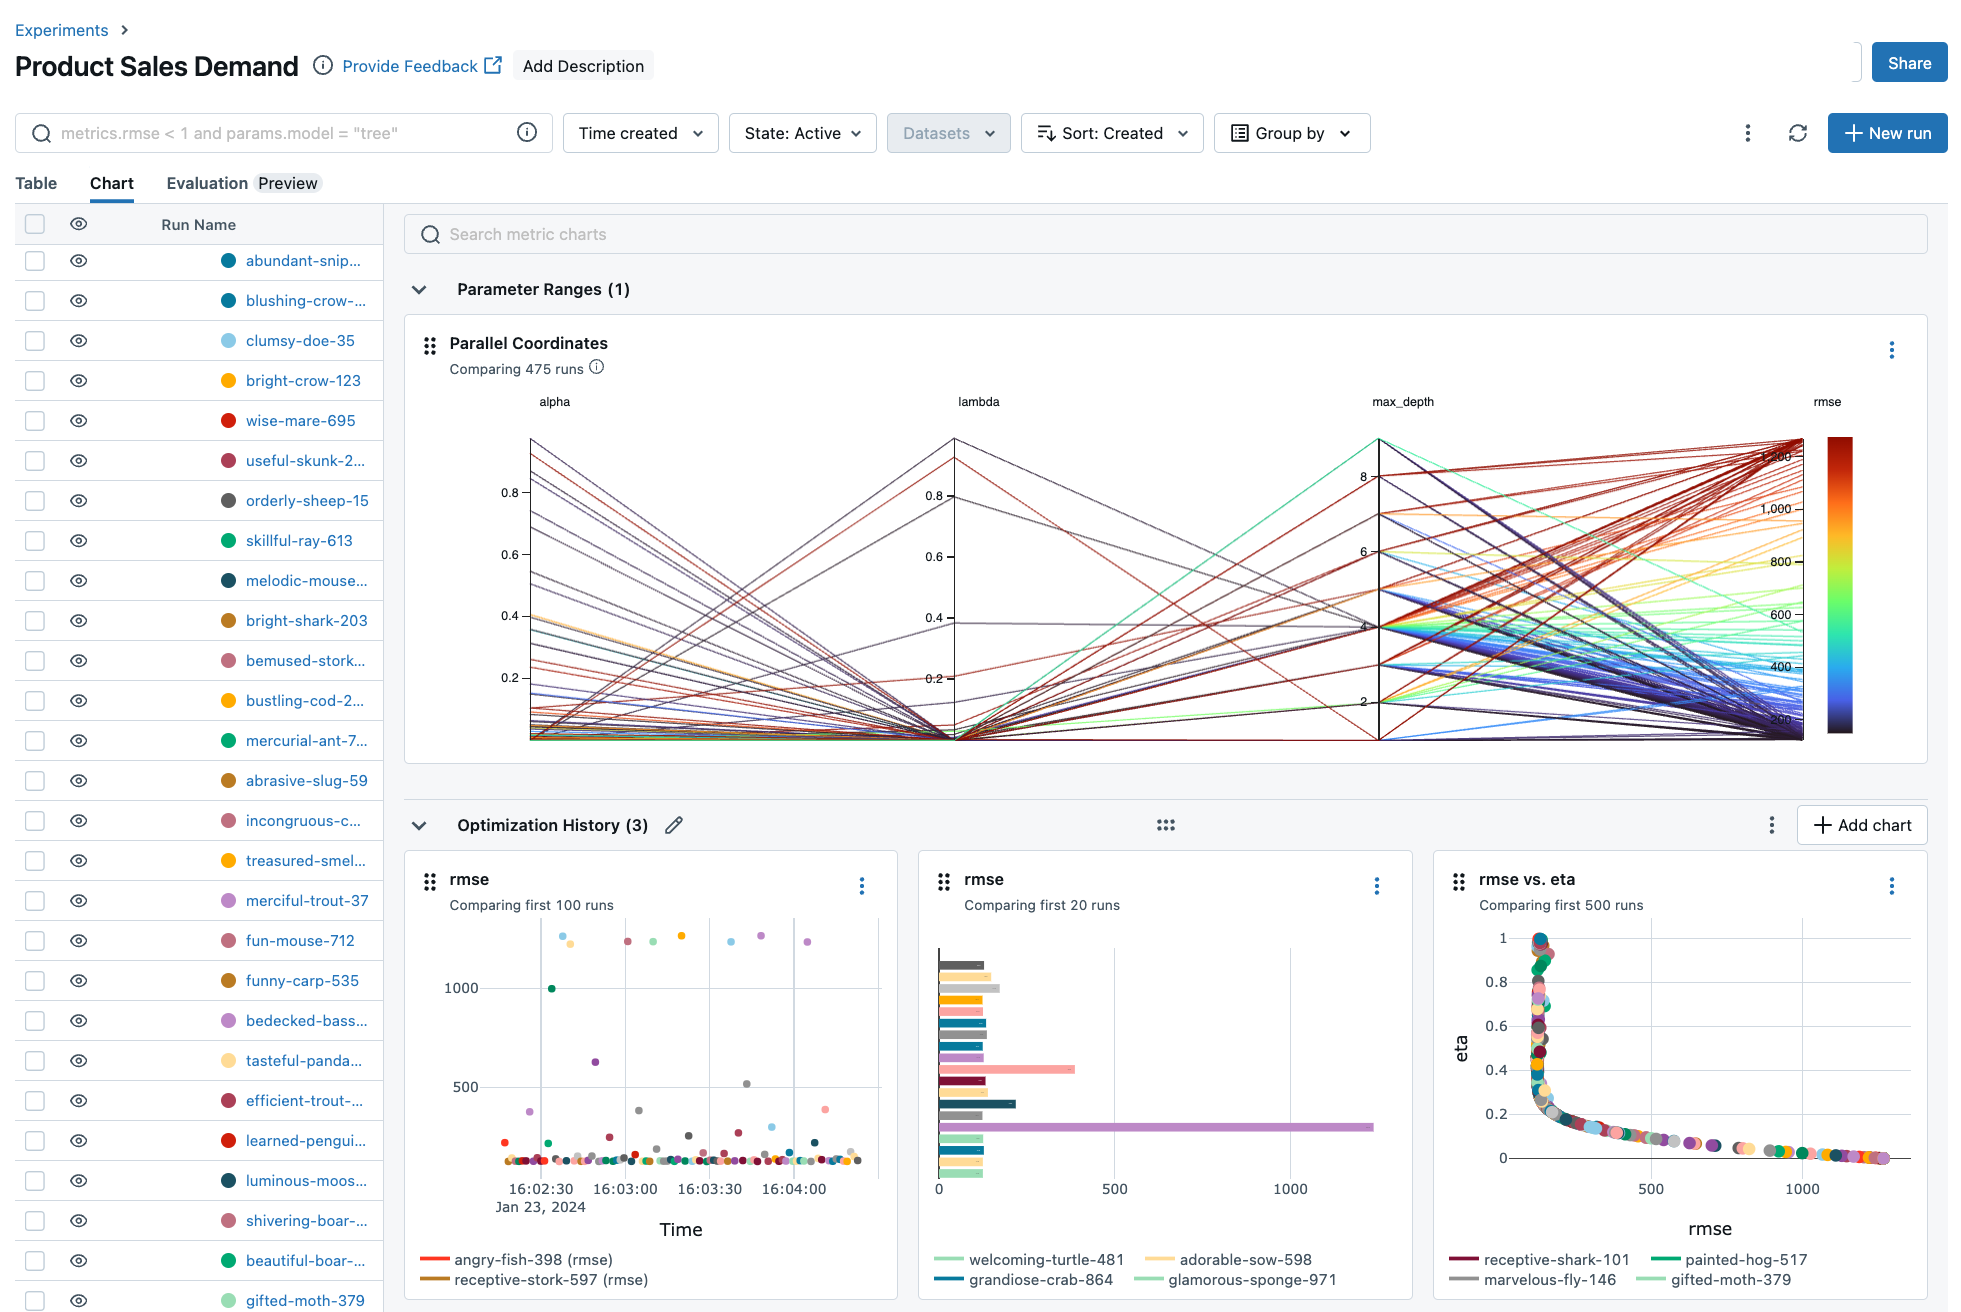
\includegraphics[width=.75\linewidth]{MLFlowSample.png}
    \caption{An example of the MLFlow monitoring dashboard \autocite{mlflow_mlflow_nodate}.}
    \label{fig:MLFlowSample}
\end{figure}

% \chapter*{Conclusion}
% \addcontentsline{toc}{chapter}{Conclusion}
% The constructed plan should provide a clear set of instructions as well as the division of tasks 
% to successfully implement the ML pipeline. It facilitates all stages of the pipeline, as well as 
% covering all of the software intended to be used, and how it will be used, at each of the stages.
% However, this plan will see continuous and repeated iteration, much like the pipeline itself, to ensure 
% that the development of the pipeline can be a smooth process without any major issues.
% In future, each stage of the perfected plan will be executed to produce an optimal MLOps pipeline, with the final 
% product being an accurate binary classification model for identifying if a person should be permitted a 
% loan from thirteen predictor variables. 


% Through the development of this plan, considerable research into machine learning operations and the literature 
% surrounding them has resulted in several skills being obtained through the discovery and use of 
% a variety of software and libraries used across data engineering industries, such as but not limited to:

% \begin{itemize}
%     \item Pandas for data analysis.
%     \item Airflow for workflow design and execution.
%     \item Docker for software containerisation.
%     \item Database management systems (MariaDB in this project) for the efficient storage of data.
%     \item Machine learning libraries (Scikit-learn in this project) 
%     \item Data validation libraries (Great Expectations)
%     \item Webserver and API libraries (Uvicorn, FastAPI) to host frontend REST APIs.
% \end{itemize}
% Side-note: I think this actually builds immensely faster because it's not recompiling those two every time,
% it just stores the processed version in the .aux files to be instantly reused.


% Apparently this can only go 500 words over the word count. You are already past that with the inclusion 
% of those two TeX files. She doesn't seem massively strict over it though, stating "it's just a module".
% 2012 + 3597 + This word count, unless you change either Datasets.tex or PipelineStages.tex.
% 5609 + This

\section{Data terminology}\label{sec:dataTerms} % Poor section title, consider something else.
This project must take into account four key elements of data handling these being data privacy, security, 
ethics and data protection laws. 

\begin{longtable}{ | p{0.2\textwidth} | p{0.7\textwidth} |}
    \hline
    \cellcolor{blue!25}Term & \cellcolor{blue!25}Description\\
    \hline
    Data privacy & An individual's ability to govern what happens to their personal data \autocite{cloudflare_what_nodate}. Personal data 
    refers to data that could be used to singularly identify someone \autocite{yang_big_2021}.\\
    \hline
    Data security & The protection of personal/sensitive information from unauthorized access, use or manipulation \autocite{ibm_security_2021}.
    This can be the physical protection of material such as hard drives, and software protections like encryption. \\
    \hline
    Data ethics & A blanket term encompassing the moral obligations of data collection, use and protection \autocite{harvard_business_school_5_2021}.
    Ethical data storage would mean that the data subjects willingly gave their data and can ask for its deletion at any point. 
    Mandated by data protection legislation. \\
    \hline 
    Big data ethics & The application of data ethics to massive datasets, concerning the implications of their collection and use on society as a whole
    \autocite{richards_big_2014}. \\ % Poor definition I think, maybe rewrite this one.
    \hline 
    General Data \newline Protection \newline Regulations (GDPR) & Legislation introduced in the EU in 2016, giving individuals significantly more 
    rights over their personal data. Data subjects most notably may request a copy of their data, the removal of their data, and to object to their data's 
    collection \autocite{ico_guide_2024}. Additionally, data must be kept secure using all available means. Companies who fail to adhere to these policies
    face significant sanctions of \euro10,000,000 or 2\% of the company's annual turnover for minor violations, or double this (\euro20,000,000, 4\% turnover)
    for major violations, whichever figure is higher. \\
    \hline
    Data Protection Act 2018 & When the UK left the EU, the GDPR no longer applied. Therefore, the UK adopted the GDPR as an amendment to its own
    Data Protection Act. There are minimal differences between the two, only that the UK's fines are in GBP rather than Euros, meaning fines go up 
    to \pounds17,500,000 or 4\% turnover \autocite{ico_enforcement_2024}. \\
    \hline
\caption{A brief overview of relevant data terminology.}\label{tab:dataTerms}
% Maybe it shouldn't be "brief". I think GDPR especially needs its own paragraph moreso than a table column.
\end{longtable}


\chapter{Implementing the MLOps Pipeline}
\section{Ethical and Legal Considerations}
The dataset was shared under an Apache 2.0 open-source licence, permitting access and modification with no restrictions
except crediting the original author \autocite{apache_apache_nodate}, meaning that there are not any ethical or legal 
considerations of note with this dataset's usage. Given that the chosen dataset also consists of synthetic data,
there are fewer necessary considerations for its use.

\subsection{Synthetic data}
% What is Synthetic Data and what are the common methods that are currently leveraged to attempt
% to perform Synthetic Data Generation?
This term has been frequently used throughout the report to describe the Loan Approval Classification Dataset, and refers to 
data that has been generated algorithmically rather than collected from a real source. However, the generation of the 
synthetic data does often depend on real data to identify patterns and trends, meaning that legislation such as GDPR is still relevant
in those scenarios because the generated data must be impossible to link back to the original subject \autocite{Lopez2022OnTL}.
An example of synthetic data generation is SMOTE, which was used in the generation of the loan dataset \autocite{zoppelleto_financial_nodate}, 
which creates synthetic data in a dataset based on the other rows as previously mentioned in Section \ref{sec:Dataset}. SMOTE will also be used in Section 
\ref{sec:ImpPreprocessing} to balance the dataset.

\subsection{Model drift}
Model drift is a phenomenon that affects deployed production machine learning models where changes in 
their environment over time affects their performance \autocite{nigenda_amazon_2022}. Model drift is not an 
immediate occurrence, and can take a long time to occur, emphasising the importance of continuous integration and deployment. 
Table \ref{tab:Drift} details the different kinds of model drift.

\begin{longtable}{ | p{0.2\textwidth} | p{0.4\textwidth} | p{0.3\textwidth} |}
    \hline
    \cellcolor{blue!25}Drift type & \cellcolor{blue!25}Description & \cellcolor{blue!25}Dataset example\\
    \hline
    Data drift & Changes in the distributions of the ingested data over time that eventually significantly differ from the model's training data \autocite{datacamp_understanding_nodate}.
    & In this dataset, interest rates and people's yearly income may change as time passes or economic inflation occurs.\\
    \hline
    Concept drift & Changes in the relationship between the input and target variables \autocite{nigenda_amazon_2022}. 
    & In this dataset, this is somewhat unlikely. However, it could occur if there is a significant housing or job market crash 
    that would cause more people to need loans, which would change the original relationships.\\
    \hline
\caption{The common types of model drift.}\label{tab:Drift}
\end{longtable}

\pagebreak % It's just barely on the same page as the table but I don't want it to be.
\para Model drift can be a significant issue that greatly impacts the performance of ML models if it is not quickly noticed, and can 
also be an ethical concern if the model is being used to influence decisions such as granting loans in this project. 
Therefore, combatting model drift through methods such as continuous monitoring is necessary to ensure that the model remains accurate 
and usable. This can be accomplished in this project through MLFlow's monitoring dashboard.

% REVIEW TASK SHEETS 2, 3 AND 4.
% NOT SURE OF THE SEQUENCE OF 3 AND 4, CHECK EXAMPLE WORK.
% Example 2 (SimonRoadknight) is 21,334 words, or 18,809 without its appendices and references.
% Example 3 (MihaiValentin) is 12,802 words.



\chapter{Implementing the MLOps Pipeline}\label{ch:Imp}

\section{Initial Software Setup}
This section details the configuration of the key software and packages within the pipeline. The installation 
processes of Miniconda and Docker are very lengthy and can therefore be found in Appendix A.

\subsection{VirtualBox \& Ubuntu}
The majority of data scientists utilise Linux distributions for their projects due to its open-source nature and the 
availability of many tools and packages. Therefore, VirtualBox, software to create a virtual machine which runs inside the host 
machine \autocite{oracle_oracle_nodate}, will be used to virtualise an Ubuntu 22.04 LTS system on the Windows host machine. This 
particular OS was chosen because it is a modern, well-supported OS with frequent software \& security updates. Virtual machines
also allow for "snapshots", which store the current state of the machine and its files at that time to be restored at any point in the 
event of unforeseen errors. Should a catastrophic error that would damage the system occur, the host machine would be unaffected as the 
virtual machine is isolated. The snapshots taken during the development of the pipeline are depicted in Figure \ref{fig:VBoxSnapshots}.

\begin{figure}[H]
    \centering
    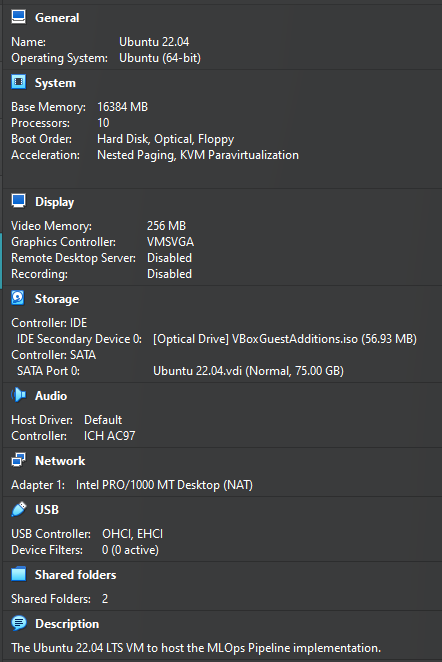
\includegraphics[width=.5\linewidth]{Implementation/VBoxConfig.png}
    \caption{The configuration for the pipeline's VM.}
    \label{fig:VBoxConfig}
\end{figure}

\begin{figure}[H]
    \centering
    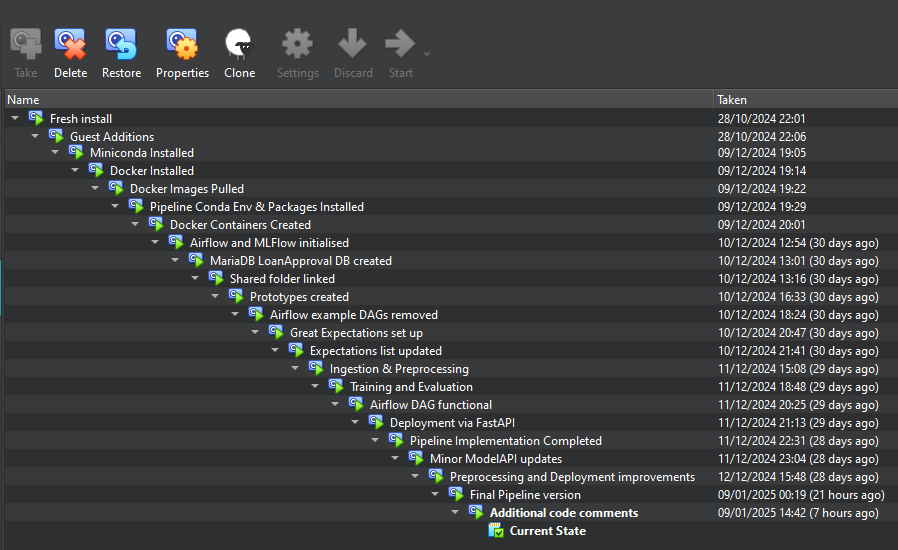
\includegraphics[width=.75\linewidth]{Implementation/JAN 10 UPDATES/VBoxSnapshots.png}
    \caption{The snapshots of the VM taken throughout the implementation.}
    \label{fig:VBoxSnapshots}
\end{figure}

\begin{figure}[H]
    \centering
    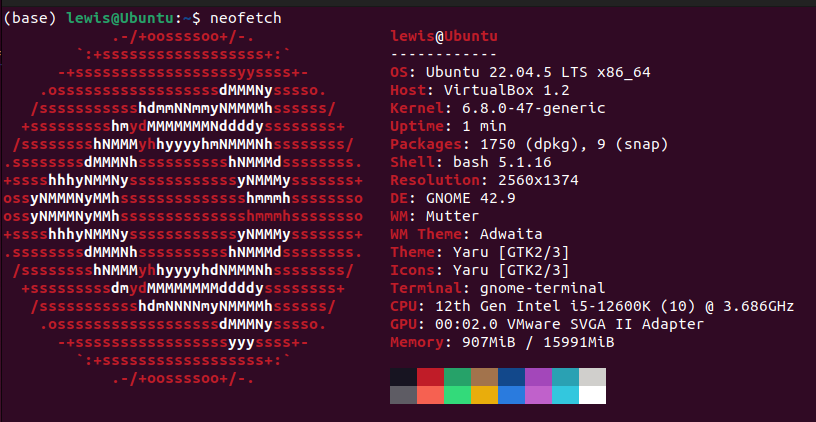
\includegraphics[width=.75\linewidth]{Implementation/Neofetch.png}
    \caption{The VM's Neofetch display.}
    \label{fig:Neofetch}
\end{figure}

\subsection{Conda environment and packages}
This section details the installation of packages to the Pipeline environment.

\begin{figure}[H]
    \centering
    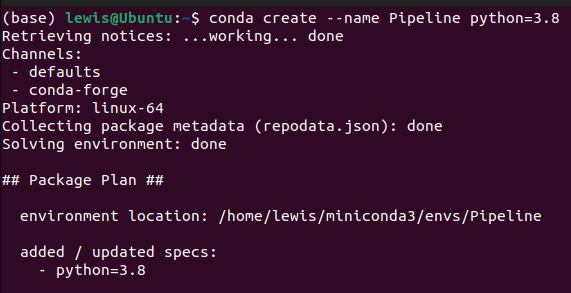
\includegraphics[width=.75\linewidth]{Implementation/Conda/CondaCreation.png}
    \caption{Creating the "Pipeline" Conda environment.}
    \label{fig:CondaCreation}
\end{figure}

\para Python 3.9.7 is used due to package compatibility issues with later versions of Python.

\begin{figure}[H]
    \centering
    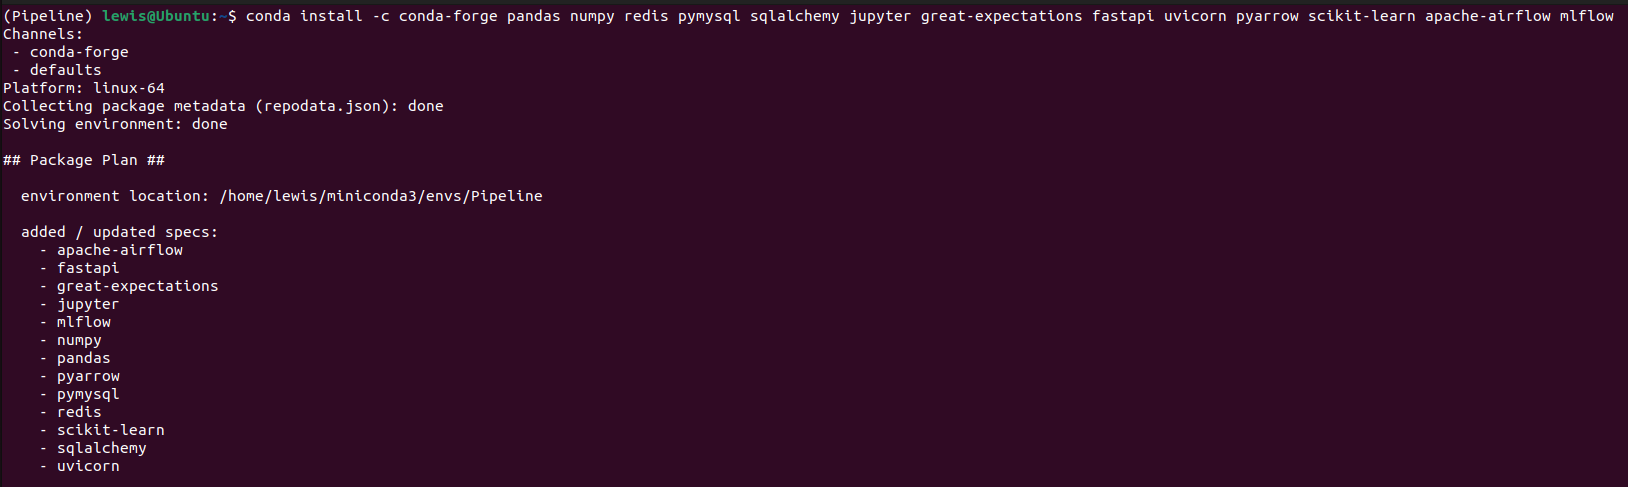
\includegraphics[width=\linewidth]{Implementation/Conda/CondaPackages.png}
    \caption{Installing packages to the environment via Conda.}
    \label{fig:CondaPackages}
\end{figure}

\para Later in development, it was discovered that three packages that were necessary were not included 
in the original install command in Figure \ref{fig:CondaPackages}. They were installed at a later point and 
detailed in Figures \ref{fig:imbLearnInstall}, \ref{fig:AirflowGXInstall}, and \ref{fig:directRedisInstall}.

\begin{figure}[H]
    \centering
    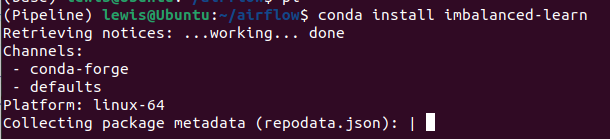
\includegraphics[width=\linewidth]{Implementation/Conda/ImbalancedLearn.png}
    \caption{Installing the imbalanced-learn package to access SMOTE.}
    \label{fig:imbLearnInstall}
\end{figure}

\begin{figure}[H]
    \centering
    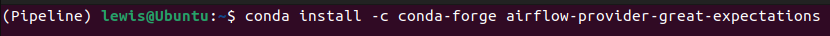
\includegraphics[width=\linewidth]{Implementation/Conda/GXAirflow.png}
    \caption{Installing the airflow-provider-great-expectations package for easy use of GX within the Airflow DAG.}
    \label{fig:AirflowGXInstall}
\end{figure}

\begin{figure}[H]
    \centering
    \includegraphics[width=\linewidth]{Implementation/Conda/DirectRedis.png}
    \caption{Installing the Direct-Redis package.}
    \label{fig:directRedisInstall}
\end{figure}

\para Direct-redis was installed via Pip, as it has not been uploaded to any Conda
channels, meaning Conda would be unable to install it.

\pagebreak 
\subsection{Docker and Docker images}
This section covers the downloading of the two necessary Docker images, MariaDB Columnstore and Redis. 
Their usage is further elaborated upon later in this chapter. The images for the containers will first need to be
downloaded from Docker's repository, shown in Figure \ref{fig:DockerPull}.

\begin{figure}[H]
    \centering
    \includegraphics[width=\linewidth]{Implementation/Docker/Containers/Pull.png}
    \caption{Pulling the Docker images.}
    \label{fig:DockerPull}
\end{figure}

\pagebreak 
\subsubsection{MariaDB Columnstore}
MariaDB Columnstore runs on port 3306, but is mapped to port 3307 to avoid a possible Docker error.

\begin{figure}[H]
    \centering
    \includegraphics[width=\linewidth]{Implementation/Docker/Containers/MariaDB/1.png}
    \caption{Creating the MariaDB Columnstore container.}
    \label{fig:CreateMCS}
\end{figure}

\begin{figure}[H]
    \centering
    \includegraphics[width=\linewidth]{Implementation/Docker/Containers/MariaDB/2.png}
    \caption{Creating the user account for MariaDB.}
    \label{fig:CreateMCSUser}
\end{figure}

\begin{figure}[H]
    \centering
    \includegraphics[width=\linewidth]{Implementation/Docker/Containers/MariaDB/3.png}
    \caption{Creating the database for later use.}
    \label{fig:CreateDB}
\end{figure}

\pagebreak 
\subsubsection{Redis}
The Docker container for Redis, the in-memory data store, is hosted on port 6379 which is the 
industry-standard default port used by the service \autocite{stream_security_security_nodate}. 
As with the Columnstore container, the Redis container can be directly interfaced with by running a 
Bash terminal inside of it. From there, the Redis command-line interface can be accessed, which confirms 
that the container's creation was successful. 

\begin{figure}[H]
    \centering
    \includegraphics[width=\linewidth]{Implementation/Docker/Containers/Redis/1.png}
    \caption{Creating and accessing the Redis container.}
    \label{fig:CreateRedis}
\end{figure}


\subsection{Airflow and MLFlow initialisation}
Airflow and MLFlow do not immediately work upon install, and must first be initialised.

\subsubsection{Airflow}
Airflow's database of DAGs can be initialised through "airflow db init", which will create 
the default Airflow directory and database file.

\begin{figure}[H]
    \centering
    \includegraphics[width=\linewidth]{Implementation/Airflow/Initialisation/1.png}
    \caption{Initialising Airflow's database.}
    \label{fig:AirflowInit}
\end{figure}

\noindent Airflow allows for the creation of user accounts with allocated permission levels for the management of 
DAGs. Therefore, an administrative user was created for the purposes of this pipeline as depicted in Figures 
\ref{fig:AirflowUser1} and \ref{fig:AirflowUser2}.

\begin{figure}[H]
    \centering
    \includegraphics[width=\linewidth]{Implementation/Airflow/Initialisation/2.png}
    \caption{Creating an administrative Airflow user.}
    \label{fig:AirflowUser1}
\end{figure}

\begin{figure}[H]
    \centering
    \includegraphics[width=\linewidth]{Implementation/Airflow/Initialisation/3.png}
    \caption{Verifying that the user was created.}
    \label{fig:AirflowUser2}
\end{figure}

\noindent After creating an admin user, the Airflow web server and task scheduler can be started. The web server provides 
an interface for reviewing DAGs, whereas the scheduler is the key backend component which executes each task within a 
DAG sequentially. Additionally, the scheduler will also automatically execute time-scheduled tasks such as those set to 
execute daily.

\begin{figure}[H]
    \centering
    \includegraphics[width=\linewidth]{Implementation/Airflow/Initialisation/4.png}
    \caption{Successfully starting Airflow's web server.}
    \label{fig:AirflowWebserver}
\end{figure}

\begin{figure}[H]
    \centering
    \includegraphics[width=\linewidth]{Implementation/Airflow/Initialisation/5.png}
    \caption{Successfully starting Airflow's task scheduler.}
    \label{fig:AirflowScheduler}
\end{figure}

\subsubsection{MLFlow}
MLFlow will be used for the continuous monitoring and storage of the produced models. 
After installing it with Conda as depicted in Figure \ref{fig:CondaPackages}, it must then 
be initialised. This is performed by creating a dedicated directory for the service and then 
creating its server.

\begin{figure}[H]
    \centering
    \includegraphics[width=\linewidth]{Implementation/MLFlow/Initialisation/1.png}
    \caption{Creating a directory for MLFlow and initialising its database.}
    \label{fig:MLFlowInit}
\end{figure}

\para To do so, the Pipeline environment must be active for MLFlow to be recognised. Then the server 
is established, setting its backend storage database as an SQLite database titled "mlflow.db",
its artifact (model) storage location as the "artifacts" subfolder, and setting the host IP as 0.0.0.0. By using 
this IP rather than localhost, it allows for applications inside containers (i.e. Airflow, Redis) to communicate 
with MLFlow when they otherwise would be unable to due to their containerisation. The database file and "artifacts"
subfolder were also created by MLFlow upon execution of the command as they did not exist at the time. 

\begin{figure}[H]
    \centering
    \includegraphics[width=\linewidth]{Implementation/MLFlow/Initialisation/3.png}
    \caption{Running MLFlow's frontend web UI.}
    \label{fig:MLFlowUICmd}
\end{figure}

\begin{figure}[H]
    \centering
    \includegraphics[width=\linewidth]{Implementation/MLFlow/Initialisation/2.png}
    \caption{MLFlow's web UI from a fresh installation.}
    \label{fig:MLFlowEmptyUI}
\end{figure}

\para The MLFlow web interface can be accessed by simply running "mlflow ui" as depicted in Figure \ref{fig:MLFlowUICmd}
and then navigating to localhost:5000 in a web browser. At present, there are no experiments or models as the software 
was freshly installed and initialised.

\subsection{Great Expectations}
Great Expectations (GX) is used for validating the dataset. It allows for the automatic processing of 
the data against rules that can be set. GX cannot be used immediately after install, and has some initialisation 
steps detailed in Figures \ref{fig:GXVersion} through \ref{fig:GXCheckpoint2}.

\begin{figure}[H]
    \centering
    \includegraphics[width=\linewidth]{Implementation/GX/Initialisation/1.png}
    \caption{Checking the installed GX version and initialising it.}
    \label{fig:GXVersion}
\end{figure}

\begin{figure}[H]
    \centering
    \includegraphics[width=\linewidth]{Implementation/GX/Initialisation/2.png}
    \caption{Confirmation of the successful initialisation.}
    \label{fig:GXInitConfirm}
\end{figure}

% \begin{figure}[H]
%     \centering
%     \includegraphics[width=\linewidth]{Implementation/GX/Initialisation/3.png}
%     \caption{Viewing the contents of the created directory.}
%     \label{fig:GXDir}
% \end{figure}

\para This pipeline uses GX version 0.18.15 as seen previously in Figure \ref{fig:GXVersion},
meaning it supports their new fluent configuration. However, this will not be necessary,
and the data source can be created from the CLI.

\begin{figure}[H]
    \centering
    \includegraphics[width=\linewidth]{Implementation/GX/Initialisation/4.png}
    \caption{Creating a new data source (1/3)}
    \label{fig:GXDatasource1}
\end{figure}

\para Upon the initial creation of the data source, GX automatically opens a Jupyter notebook for its 
configuration, depicted below in Figure \ref{fig:GXDatasource2}. Part of the creation process 
involves naming the data source, and therefore "LoanApproval\_DataSource" was used as the name.

\begin{figure}[H]
    \centering
    \includegraphics[width=\linewidth]{Implementation/GX/Initialisation/5.png}
    \caption{Creating a new data source (2/3)}
    \label{fig:GXDatasource2}
\end{figure}

\para Towards the end of the configuration notebook, there is a block containing two functions, where the first 
will ensure that the configuration is sanitised and valid where it is then saved, and the second is to output the created 
data source's properties to ensure they match what was expected.

\begin{figure}[H]
    \centering
    \includegraphics[width=\linewidth]{Implementation/GX/Initialisation/6.png}
    \caption{Creating a new data source (3/3)}
    \label{fig:GXDatasource3}
\end{figure}

\para The output text matched what was expected of the data source, meaning that the data source is finalised
and ready to use. Next, a "suite" must be created to allow for the easy creation of expectations \autocite{gx_expectation_nodate}.
The creation process is similar to that of the data source, where the command is executed, and configuration details are confirmed in 
a Jupyter notebook as depicted in Figure \ref{fig:GXSuite2}.

\begin{figure}[H]
    \centering
    \includegraphics[width=\linewidth]{Implementation/GX/Initialisation/7.png}
    \caption{Creating a new suite (1/2)}
    \label{fig:GXSuite1}
\end{figure}

\begin{figure}[H]
    \centering
    \includegraphics[width=.75\linewidth]{Implementation/GX/Initialisation/8.png}
    \caption{Creating a new suite (2/2). The full list of expectations is in Table \ref{tab:Expectations}.}
    \label{fig:GXSuite2}
\end{figure}

\begin{longtable}{ | p{0.4\textwidth} | p{0.5\textwidth} |}
    \hline
    \cellcolor{blue!25}Item & \cellcolor{blue!25}Expectation\\
    \hline
    Dataset & Must be exactly 14 columns. \\
    \hline
    loan\_status & Must not be null. \newline Must be 0 or 1. \\
    \hline 
    person\_gender & Must be 'female' or 'male'. \\
    \hline 
    person\_education & Must be 'Bachelor', 'Associate', 'High School', 'Master', or 'Doctorate'. \\
    \hline
    person\_home\_ownership & Must be 'RENT', 'MORTGAGE', 'OWN', or 'OTHER'.\\
    \hline 
    loan\_intent & Must be 'EDUCATION', 'MEDICAL', 'VENTURE', 'PERSONAL', 'DEBTCONSOLIDATION', or 'HOMEIMPROVEMENT'.\\
    \hline 
    previous\_loan\_defaults\_on\_file & Must be 'Yes' or 'No'. \\
    \hline
    credit\_score & Must be between 350 and 900. \\
    \hline
    cb\_person\_cred\_hist\_length & Must be between 0 and 30. \\
    \hline
    loan\_percent\_income & Must be between 0 and 0.8. \\
    \hline
    loan\_int\_rate & Must be between 5.0 and 30.0. \\
    \hline
    loan\_amnt & Must be between 0 and 50,000. \\
    \hline 
    person\_emp\_exp & Must be between 0 and 125. \\
    \hline 
    person\_income & Must be greater than 5000. \\
    \hline 
    person\_age & Must be greater than 0. \\
    \hline
\caption{Expectations set for the dataset and its columns.}\label{tab:Expectations}
\end{longtable}

\para After the suite's creation, GX then allows for the creation of checkpoints, which save the expectations and allow
them to be applied to any dataset, which would be useful when the dataset is updated, as there would be no need 
to create a new suite of expectations.

\begin{figure}[H]
    \centering
    \includegraphics[width=.75\linewidth]{Implementation/GX/Initialisation/9.png}
    \caption{Creating the checkpoint based on the suite.}
    \label{fig:GXCheckpoint1}
\end{figure}

\noindent As with the data source and suite, a Jupyter Notebook is opened upon the checkpoint's creation, giving a final overview 
of the properties of the checkpoint such as its name, connected data source and connected suite. The final block of the 
notebook (Figure \ref{fig:GXCheckpoint2}) saves the checkpoint to a YAML file (Figure \ref{fig:GXCheckpoint3}) and outputs
the properties which were confirmed to be correct. 

\begin{figure}[H]
    \centering
    \includegraphics[width=.75\linewidth]{Implementation/GX/Initialisation/10.png}
    \caption{Saving the checkpoint in the prompted Jupyter notebook.}
    \label{fig:GXCheckpoint2}
\end{figure}

\begin{figure}[H]
    \centering
    \includegraphics[width=.75\linewidth]{Implementation/GX/Initialisation/11.png}
    \caption{Confirming the existence of the checkpoint YAML file.}
    \label{fig:GXCheckpoint3}
\end{figure}

\section{Package imports}\label{sec:PkgImports}
Many packages need to be imported for the Airflow DAG of the pipeline to succeed. These can be found 
below, alongside descriptions in the form of Python comments, in Figures \ref{fig:PipelineDAGImports} and 
\ref{fig:PipelineFunctionsImports}. The use of these packages within pipeline functions is detailed 
in this report within the appropriate pipeline stage.

\begin{figure}[H]
    \centering
    \includegraphics[width=\linewidth]{Implementation/.Code/PipelineDAGImports.png}
    \caption{The packages necessary to run the DAG itself.}
    \label{fig:PipelineDAGImports}
\end{figure}

\begin{figure}[H]
    \centering
    \includegraphics[width=\linewidth]{Implementation/.Code/PipelineFunctionsImport.png}
    \caption{The packages necessary to run the functions within each DAG.}
    \label{fig:PipelineFunctionsImports}
\end{figure}
% Elements of SoftwareInit could be placed in the appropriate pipeline section.

\section{Package imports}
Many packages need to be imported for the Airflow DAG of the pipeline to succeed. These can be found 
below, alongside descriptions in the form of Python comments, in Figures \ref{fig:PipelineDAGImports} and 
\ref{fig:PipelineFunctionsImports}. The use of these packages within pipeline functions is detailed 
in this report within the appropriate pipeline stage.

\begin{figure}[H]
    \centering
    \includegraphics[width=\linewidth]{Implementation/.Code/PipelineDAGImports.png}
    \caption{The packages necessary to run the DAG itself.}
    \label{fig:PipelineDAGImports}
\end{figure}

\begin{figure}[H]
    \centering
    \includegraphics[width=\linewidth]{Implementation/.Code/PipelineDAGImports.png}
    \caption{The packages necessary to run the functions within each DAG.}
    \label{fig:PipelineFunctionsImports}
\end{figure}

\section{Data Ingestion}\label{sec:ImpIngestion}

\begin{figure}[H]
    \centering
    \includegraphics[width=\linewidth]{Implementation/.Code/PipelineFunctions/Ingestion.png}
    \caption{The code for the entire Ingestion stage.}
    \label{fig:IngestionCode}
\end{figure}

\para This code is split across four functions that are called upon within the main 
ETL function. The ETL function will call on extract\_csv to read the dataset CSV from 
the path set as DEFAULT\_PATH. After this, some data type transformations are performed 
to ensure the optimal data types are used for each column. Finally, the transformed 
Pandas DataFrame is written to the MariaDB Columnstore instance hosted within the Docker 
container at port 3306.

\para For data validation,
Conda was used to install a helper package for Airflow that adds the Great Expectations Operator.
This operator connects to the checkpoint produced in Figure \ref{fig:GXCheckpoint3} to run the saved validation 
methods on the ingested dataset without the need to declare it as a specialised Python function within 
the code. 

\section{Data Preprocessing}\label{sec:ImpPreprocessing}

\begin{figure}[H]
    \centering
    \includegraphics[width=\linewidth]{Implementation/.Code/PipelineFunctions/Preprocessing1.png}
    \caption{The secondary functions used in the main Preprocessing function.}
    \label{fig:PreprocessingCode1}
\end{figure}

\begin{figure}[H]
    \centering
    \includegraphics[width=\linewidth]{Implementation/.Code/PipelineFunctions/Preprocessing2.png}
    \caption{The code for the main Preprocessing function.}
    \label{fig:PreprocessingCode2}
\end{figure}

\para This code forms the Data Preprocessing stage of the pipeline. Data is retrieved from the 
Columnstore and considerable outliers are removed, primarily from the Age and Income columns, 
where data can be outright false or differs enough to heavily skew the dataset and affect scaling.
After this, categorical data is encoded using label encoding and one-hot encoding where necessary.
The data is then balanced using SMOTE to resolve the significant imbalance between granted and denied loans 
before being split into training and testing sets, which are serialized and saved into Redis. The use of 
a DirectRedis connection rather than a standard Redis connection removes the need for explicit serialization, 
as it is automatically performed when "r.set()" is called. 

\section{Model Development}\label{sec:ImpDevelopment}
Internally, this section was referred to as "Training", seen in the function name and associated 
DAG task.

\begin{figure}[H]
    \centering
    \includegraphics[width=\linewidth]{Implementation/.Code/PipelineFunctions/Training.png}
    \caption{The code for the Training function.}
    \label{fig:TrainingCode}
\end{figure}

The Training function deserializes and reads the preprocessed DataFrame from Redis via a Direct-Redis 
connection, and then scales the data using a StandardScaler from Scikit-Learn. MLFlow is started 
to begin its tracking of the model, and then the model is instantiated and trained on the preprocessed data 
using the parameters provided to the Training function. These parameters would be provided within the DAG code.
The model is then serialized using Pickle and stored into Redis, alongside the parameters for logging purposes 
and the MLFlow run ID so that the run can be resumed in the Evaluation phase.


\section{Model Evaluation}\label{sec:ImpEvaluation}

\begin{figure}[H]
    \centering
    \includegraphics[width=\linewidth]{Implementation/.Code/PipelineFunctions/Evaluation1.png}
    \caption{eval\_metrics, which returns the evaluation metrics of a model.}
    \label{fig:Evaluation1}
\end{figure}

\para The eval\_metrics function calculates the accuracy, precision and F1 scores of the trained model 
using predefined functions that are part of Scikit-Learn. This is later used in the main Evaluation function 
to log these scores in MLFlow.

\begin{figure}[H]
    \centering
    \includegraphics[width=\linewidth]{Implementation/.Code/PipelineFunctions/Evaluation2.png}
    \caption{The main Evaluation function.}
    \label{fig:Evaluation2}
\end{figure}

\para The Evaluation function retrieves the serialized model, parameters and run ID from Redis 
via a Direct-Redis connection, deserializing the model with Pickle. The testing dataset is 
retrieved and the MLFlow run is resumed to then make predictions using the model. Using the 
eval\_metrics function, the metrics obtained are output to the console (viewable via the DAG's logs page)
and also logged in the MLFlow run. The model is then saved and the MLFlow is ended, completing the pipeline.

\section{Completed Airflow DAGs}
Two DAGs were created as part of the pipeline. "DockerContainers" consists of two BashOperators 
to start the two Docker containers for MariaDB Columnstore and Redis, whereas "MLOpsPipeline" 
consists of the five tasks of the pipeline. Figure \ref{fig:DAGsList} shows the list of DAGs, 
containing only these two\footnote{Normally, Airflow includes a large list of examples, though these were 
removed by changing the configuration file located at \texttildelow/airflow/airflow.cfg.} DAGs.

\begin{figure}[H]
    \centering
    \includegraphics[width=\linewidth]{Implementation/Airflow/DAGs/1.png}
    \caption{The list of DAGs in Airflow.}
    \label{fig:DAGsList}
\end{figure}

\section{Pipeline}
Figure \ref{fig:PipelineGraphDAG} shows the completed Airflow DAG's graph view, which is a graphical 
representation of the sequence of tasks. The five tasks of the pipeline are shown, 
though deployment is not one of them, which is further explained in Section \ref{sec:ImpDeployment}.

\begin{figure}[H]
    \centering
    \includegraphics[width=\linewidth]{Implementation/Airflow/DAGs/PipelineGraph.png}
    \caption{The graph view of the completed MLOpsPipeline DAG.}
    \label{fig:PipelineGraphDAG}
\end{figure}

The code for the completed DAG consists of four PythonOperators, each to call the respective main 
function of each stage as detailed in their respective section, as well as a GreatExpectationsOperator 
to run data validation between ingestion and preprocessing. It also declares some variables that are passed 
to each function, which can be easily modified.

\begin{figure}[H]
    \centering
    \includegraphics[width=\linewidth]{Implementation/.Code/PipelineDAG.png}
    \caption{The complete code of the MLOpsPipeline DAG.}
    \label{fig:PipelineDAGCode}
\end{figure}


\section{Model Deployment}\label{sec:ImpDeployment}
Deployment is performed separately from the rest of the stages in this pipeline, 
as it involves the hosting of a Uvicorn server on port 8000 to run the code written 
in the Model API script using FastAPI. Through running the server using the command 
"uvicorn modelAPI:main --reload" as detailed in Figure 
\ref{fig:UviStartup}, the "docs" page of FastAPI can be accessed to manually perform POST 
requests to get predictions from the model. The "--reload" argument means that whenever the 
modelAPI Python file is updated, the server will automatically update it with the changes.

\begin{figure}[H]
    \centering
    \includegraphics[width=\linewidth]{Implementation/FastAPI+Uvi/Startup.png}
    \caption{Starting the Uvicorn server on port 8000.}
    \label{fig:UviStartup}
\end{figure}

\begin{figure}[H]
    \centering
    \includegraphics[width=\linewidth]{Implementation/FastAPI+Uvi/LoadModel.png}
    \caption{Loading the pickled model to make predictions with.}
    \label{fig:UviLoadModel}
\end{figure}

\begin{figure}[H]
    \centering
    \includegraphics[width=.5\linewidth]{Implementation/FastAPI+Uvi/InputAndPrediction.png}
    \caption{The FastAPI classes used for input and predictions.}
    \label{fig:UviClasses}
\end{figure}

\begin{figure}[H]
    \centering
    \includegraphics[width=\linewidth]{Implementation/FastAPI+Uvi/Code.png}
    \caption{The FastAPI endpoints for getting model predictions.}
    \label{fig:UviCode}
\end{figure}

\para The docs page generated from these endpoints is shown below in Figure \ref{fig:UviDocs}.
Using this page, inputs can be given to the model by making a POST request to its endpoint, 
which will return a prediction.

\begin{figure}[H]
    \centering
    \includegraphics[width=\linewidth]{Implementation/FastAPI+Uvi/DocsPage.png}
    \caption{The docs page for the model-API script.}
    \label{fig:UviDocs}
\end{figure}

\para POST requests can be made by clicking on the endpoint "/loan/predict/single",
followed by "Try it out" and then entering data for each row. The model will then 
interpret the data for each column and make a prediction based upon it. To test this, 
two predictions were given to the model, where one is a loan that would be granted (Figure \ref{fig:UviTruePositive})
and the other is a loan that would not be granted (Figure \ref{fig:UviTrueNegative}). 

\begin{figure}[H]
    \centering
    \includegraphics[width=\linewidth]{Implementation/FastAPI+Uvi/TruePositive.png}
    \caption{The response for a loan that would be granted (loan\_status of 1).}
    \label{fig:UviTruePositive}
\end{figure}

\begin{figure}[H]
    \centering
    \includegraphics[width=\linewidth]{Implementation/FastAPI+Uvi/TrueNegative.png}
    \caption{The response for a loan that would be rejected (loan\_status of 0).}
    \label{fig:UviTrueNegative}
\end{figure}

\para Both of these inputs were correctly predicted, which is known because they were 
two rows from the dataset.



\section{Potential security enhancements}\label{sec:SecurityEnhancements}
In relation to Model Deployment, it is important to note that the use of the "docs" page is not suitable for an actual production 
environment, as it can be manipulated by threat actors to possibly give them direct access to the 
server's backend, meaning it is normally disabled. An actual production environment would link their 
model to their actual web page with forms and text entry fields to input data, though this would not 
have been feasible for this particular project due to time constraints as well as not owning a domain 
to host the site on, meaning it is restricted to only localhost.


\section{Development challenges and future improvements}
During the implementation of the pipeline, the initial package used for serializing data was PyArrow.
However, as development continued, it was discovered that many of PyArrow's useful functions are now 
deprecated, and have been since 2021. This made serializing data and passing it between DAG stages considerably more difficult, 
and for this reason an alternative package was identified: Direct-Redis. Direct-Redis builds on top of the Redis 
package, but will instantly serialize and deserialize data when set() or get() is called, greatly expediting 
the process of storing data in and retrieving data from Redis stores. \autocite{direct-redis_direct-redis_nodate}.
This resolved the serialization issue, meaning the pipeline worked smoothly without any errors, and also 
resulted in much cleaner and easily-readable code. An alternative which would have also worked would have been to 
use Pickle for all serialization rather than just that of the model, which would have been functionally identical.

\para Additionally, during the preprocessing stage, a minor improvement could have been made with the One-Hot 
encoding of the "previous\_loan\_defaults\_on\_file" column by removing the "Yes" column it produces, because 
if one is 0, the other must be 1, meaning that two columns are not needed.

\para Furthermore, the DAG that starts the Docker containers could also be extended to add a BashOperator to run 
"mlflow ui" to initialise the MLFlow server. Currently, just running the DockerContainers DAG followed by the pipeline DAG will 
time out unless MLFlow was already running because the Training and Evaluation phases are unable to connect to MLFlow 
if it is not running.

\para Finally, it could theoretically be possible to incorporate deployment within the DAG through the use of a 
BashOperator to run "uvicorn modelAPI:app --reload". However, this may lead to issues with directories which will be 
looked into, as well as the DAG never actually ending, and running perpetually because the Uvicorn server will not stop 
by itself. On the topic of deployment, the user needing to enter 24 columns of data as a result of One-Hot encoding 
increasing the dimensionality is poor, and encoding the data \textbf{after it has been input} by the user is being considered so 
that the user only needs to enter the original 13 columns which will be silently encoded in the background for the model's use.

\para These issues will be resolved in the final version of the pipeline for January 10, and this section will either 
be removed or rewritten for that version of the report. 

\chapter*{Conclusion}
\addcontentsline{toc}{chapter}{Conclusion}
% REWRITE THE INTRODUCTION AFTER THIS.

% =========================================================================
% MAIN NOTES:
% 
% You need to put figures of all these screenshots in that were taken last night.
% That's screenshots from the following folders:
%   Entire .Code folder   
%   Airflow/DAGs folder 
%   Entire FastAPI+Uvi folder
%   MLFlow/Other folder.
% Uvi Code doesn't have the GET function completed? Maybe it does but I don't think so.
% Screenshot of GX Operator install needed.

% Your ingestion isn't really ingesting. Import Kaggle and download + extract the zip through the Kaggle package and a ZIP extractor package.
% Misunderstanding of Label and Ordinal encoding. Pinned a bookmark to Firefox explaining the two.
% Alternatively, with one-hot encoding, just remove the Previous_loan_defaults_no column, as if that's 0, the other must be 1.
% You may have been able to label encode the whole dataset, as random forest can apparently work well with it anyway.]

% Maybe transform the data within the modelAPI script so you don't need to enter 24 columns for a prediction.

% Detailed description on why Arrow didn't work and why Direct-Redis did. Why is Direct-Redis a pip install?
% Add a BashOperator for mlflow ui.
% Data analysis is worth 20%. Consider investing more into that section and/or moving it into the implementation chapter.

% Pipeline plan = 20%
% Implementation & Deployment = 20%
% Application & Analysis = 20%
% Evaluation & Communication of wider issues = 20%

% Remember that some of these can be implemented for Jan 10 rather than now.
% Deadline extended to Dec 19. Coincides too heavily with CMP6202 so not feasible.
% I still THOROUGHLY AND HEAVILY recommend you do it for DEC 13!
% While you could submit and proofread on 19, do not plan around leaving it until then.

% You've said the docs page is a security threat. That's true, but give a source to say that.

% Word count is likely to be approx 11,000, though there's not a massive amount you can do
% about that without slashing entire sections.

% =========================================================================
\chapter*{Appendix A - Software Installation}
\addcontentsline{toc}{chapter}{Appendix A - Software Installation}
\section*{Miniconda}

\begin{figure}[H]
    \centering
    \includegraphics[width=.75\linewidth]{Implementation/Conda/Installation/1.png}
    \caption{Getting the latest Miniconda installation script.}
    \label{fig:CondaInstall1}
\end{figure}

\begin{figure}[H]
    \centering
    \includegraphics[width=.75\linewidth]{Implementation/Conda/Installation/2.png}
    \caption{Executing the Miniconda installation script.}
    \label{fig:CondaInstall2}
\end{figure}

% \begin{figure}[H]
%     \centering
%     \includegraphics[width=.75\linewidth]{Implementation/Conda/Installation/3.png}
%     \caption{Agreeing to Miniconda's license terms.}
%     \label{fig:CondaInstall3}
% \end{figure}

\begin{figure}[H]
    \centering
    \includegraphics[width=.75\linewidth]{Implementation/Conda/Installation/4.png}
    \caption{Making Conda run automatically in all shells.}
    \label{fig:CondaInstall4}
\end{figure}

\begin{figure}[H]
    \centering
    \includegraphics[width=.75\linewidth]{Implementation/Conda/Installation/6.png}
    \caption{Adding conda-forge as a channel for package retrieval.}
    \label{fig:CondaInstall6}
\end{figure}

\pagebreak 
\section*{Docker}
Docker's install process on a fresh Ubuntu system is quite lengthy due to a lot of 
system configuration being required. This installation process follows 
\textcite{digitalocean_how_nodate}'s guide.

\begin{figure}[H]
    \centering
    \includegraphics[width=\linewidth]{Implementation/Docker/Installation/1.png}
    \caption{Installing HTTPS certificates.}
    \label{fig:DockerInstall1}
\end{figure}

\begin{figure}[H]
    \centering
    \includegraphics[width=\linewidth]{Implementation/Docker/Installation/2.png}
    \caption{Adding Docker's public GPG key for checksum validation.}
    \label{fig:DockerInstall2}
\end{figure}

\begin{figure}[H]
    \centering
    \includegraphics[width=\linewidth]{Implementation/Docker/Installation/3.png}
    \caption{Adding Docker's download page to Ubuntu's list of package repositories.}
    \label{fig:DockerInstall3}
\end{figure}

\begin{figure}[H]
    \centering
    \includegraphics[width=\linewidth]{Implementation/Docker/Installation/4.png}
    \caption{Checking if Docker is installed, which it is not.}
    \label{fig:DockerInstall4}
\end{figure}

\begin{figure}[H]
    \centering
    \includegraphics[width=\linewidth]{Implementation/Docker/Installation/5.png}
    \caption{Installing Docker.}
    \label{fig:DockerInstall5}
\end{figure}

\begin{figure}[H]
    \centering
    \includegraphics[width=\linewidth]{Implementation/Docker/Installation/6.png}
    \caption{Confirming that the Docker service is running.}
    \label{fig:DockerInstall6}
\end{figure}

\begin{figure}[H]
    \centering
    \includegraphics[width=\linewidth]{Implementation/Docker/Installation/7.png}
    \caption{Adding the VM user to the Docker group so they can execute commands.}
    \label{fig:DockerInstall7}
\end{figure}


\printbibliography

\end{document}

